\documentclass[xcolor=dvipsnames]{beamer}
%\documentclass[pdftex,hyperref={colorlinks=false}]{beamer}
%\documentclass[handout,xcolor=dvipsnames,pdftex,hyperref={colorlinks=false}]{beamer}

% == Packages for beamer
\usepackage{xcolor}
\usepackage{graphicx}
\usepackage{fancybox}
\usepackage{hyperref}
\usepackage{amsmath,amssymb,amsfonts,bm}
\usepackage{wasysym}
\usepackage{colortbl}
\usepackage[english]{babel}
\usepackage{times}
\usepackage[T1]{fontenc}
\usepackage{multirow}

% == Other Packages
\usepackage{rotating}
\usepackage{latexsym}
\usepackage{ulem}

\newenvironment{Shaded}{}{}


% == theme & colors
\usetheme{Warsaw}  % Jens' previous
\usepackage{helvet}
\definecolor{someblue}{rgb}{0,.1,0.8}

% == New Commands
% = For general typesetting
\newcommand\spacingset[1]{\renewcommand{\baselinestretch}{#1}\small\normalsize}
\renewcommand\r{\right}
\renewcommand\l{\left}

\newcommand\makegaps{\addtolength{\itemsep}{.25\baselineskip}}
\newcommand\makebiggaps{\addtolength{\itemsep}{.5\baselineskip}}
\newcommand\smallunskip{\vspace{-.25\baselineskip}}
\newcommand\medunskip{\vspace{-.5\baselineskip}}
\newcommand\bigunskip{\vspace{-\baselineskip}}

\newcommand{\VerbBar}{|}
\newcommand{\VERB}{\Verb[commandchars=\\\{\}]}
% Add ',fontsize=\small' for more characters per line
\newcommand{\KeywordTok}[1]{\textcolor[rgb]{0.00,0.44,0.13}{\textbf{{#1}}}}
\newcommand{\DataTypeTok}[1]{\textcolor[rgb]{0.56,0.13,0.00}{{#1}}}
\newcommand{\DecValTok}[1]{\textcolor[rgb]{0.25,0.63,0.44}{{#1}}}
\newcommand{\BaseNTok}[1]{\textcolor[rgb]{0.25,0.63,0.44}{{#1}}}
\newcommand{\FloatTok}[1]{\textcolor[rgb]{0.25,0.63,0.44}{{#1}}}
\newcommand{\CharTok}[1]{\textcolor[rgb]{0.25,0.44,0.63}{{#1}}}
\newcommand{\StringTok}[1]{\textcolor[rgb]{0.25,0.44,0.63}{{#1}}}
\newcommand{\CommentTok}[1]{\textcolor[rgb]{0.38,0.63,0.69}{\textit{{#1}}}}
\newcommand{\OtherTok}[1]{\textcolor[rgb]{0.00,0.44,0.13}{{#1}}}
\newcommand{\AlertTok}[1]{\textcolor[rgb]{1.00,0.00,0.00}{\textbf{{#1}}}}
\newcommand{\FunctionTok}[1]{\textcolor[rgb]{0.02,0.16,0.49}{{#1}}}
\newcommand{\RegionMarkerTok}[1]{{#1}}
\newcommand{\ErrorTok}[1]{\textcolor[rgb]{1.00,0.00,0.00}{\textbf{{#1}}}}
\newcommand{\NormalTok}[1]{{#1}}


% = For stats & econometrics
\renewcommand{\epsilon}{\varepsilon}
\newcommand\ud{\mathrm{d}}
\newcommand\dist{\buildrel\rm d\over\sim}
\newcommand\ind{\stackrel{\rm indep.}{\sim}}
\newcommand\iid{\stackrel{\rm i.i.d.}{\sim}}
\newcommand\logit{{\rm logit}}
\newcommand\cA{\mathcal{A}}
\newcommand\cN{\mathcal{N}}
\newcommand\E{\mathbb{E}}
\newcommand\V{\mathbb{V}}
\newcommand\cJ{\mathcal{J}}
\newcommand\y{{\bm y}}
\newcommand\Y{{\bm Y}}
\newcommand\X{{\bm X}}
\newcommand\x{{\bm x}}
\newcommand\eps{{\bm\varepsilon}}
\newcommand\zero{{\bm 0}}
\newcommand\be{{\bm\beta}}
\renewcommand\b{{\bm b}}
\newcommand\C{{\bm C}}
\newcommand\D{{\bm D}}
\newcommand\I{{\bm I}}
\newcommand\Z{{\bm Z}}
\newcommand\eeta{{\bm \eta}}
\newcommand{\Var}{\mathrm{Var}}
\newcommand{\Cov}{\mathrm{Cov}}

\DeclareMathOperator*\plim{plim}
\DeclareMathOperator\rank{rank}
\newcommand\indep{\protect\mathpalette{\protect\independenT}{\perp}}
\DeclareMathOperator{\sgn}{sgn}
\def\independenT#1#2{\mathrel{\rlap{$#1#2$}\mkern2mu{#1#2}}}

%\documentclass[xcolor=dvipsnames]{beamer}
%%\usecolortheme[named=OliveGreen]{structure}
%\usecolortheme[named=Blue]{structure}
%%\usetheme{Rochester}
%\setbeamertemplate{items}[ball]
%\setbeamertemplate{blocks}[rounded][shadow=true]
%\usepackage{xcolor}
%\usepackage{colortbl}
%\setbeamertemplate{navigation symbols}{}
%\usepackage{amssymb}
%\usepackage{amsmath}
%\usepackage[english]{babel}
%% or whatever
%
%%\usepackage[latin1]{inputenc}
%% or whatever
%
%%\mode<presentation>
%%{
%\usetheme{Warsaw}
%  % or ...
%  %\usecolorheme{albatross}
%%  \setbeamercovered{transparent}
%  % or whatever (possibly just delete it)
%%}

%\usepackage{helvet}
%%\usepackage[T1]{fontenc}
%% Or whatever. Note that the encoding and the font should match. If T1
%% does not look nice, try deleting the line with the fontenc.

\newtheorem{assumption}{Assumption}
\newtheorem{iass}{Identification Assumption}
\newtheorem{ires}{Identfication Result}
\newtheorem{estm}{Estimand}
\newtheorem{esti}{Estimator}

%\newcommand{\indep}{{\bot\negthickspace\negthickspace\bot}}
\newcommand{\notindep}{{\bot\negthickspace\negthickspace\bot}{\negthinspace
  \negmedspace \negthickspace \negthickspace \diagup
  \;}}

\newcommand{\bs}{\boldsymbol}
\newcommand{\mb}{\mathbf}
\newcommand{\real}{\mathbb{R}}
\renewcommand{\u}{\ensuremath{\mb{u}}}
\renewcommand{\v}{\ensuremath{\mb{v}}}
\newcommand{\U}{\ensuremath{\mb{U}}}
\newcommand{\M}{\ensuremath{\mb{M}}}
\renewcommand{\b}{\ensuremath{\bs{\beta}}}
\newcommand{\e}{\ensuremath{\bs{\epsilon}}}
\newcommand{\bhat}{\ensuremath{\hat{\bs{\beta}}}}
\newcommand{\XX}{\ensuremath{\X'\X}}
\newcommand{\XXinv}{\ensuremath{\left(\XX\right)^{-1}}}
\newcommand{\hatsig}{\ensuremath{\hat{\sigma}^2}}
\newcommand{\sig}{\ensuremath{\sigma^2}}
\newcommand{\hatmat}{\ensuremath{\X \XXinv \X'}}
\newcommand{\ehat}{\ensuremath{\hat{\e}}}
\newcommand{\tr}{\text{tr}}
\newcommand{\Sig}{\ensuremath{\bs{\Sigma}}}
\newcommand{\SigInv}{\ensuremath{\bs{\Sigma^{-1}}}}
\newcommand{\W}{\ensuremath{\mb{W}}}

%\usepackage{fixltx2e} % provides \textsubscript
%\ifxetex
%%  \usepackage{fontspec,xltxtra,xunicode}
%  \usepackage{mathspec,xltxtra,xunicode}
%  \defaultfontfeatures{Mapping=tex-text,Scale=MatchLowercase}
%  \setmainfont[Ligatures={Common,TeX}]{Gill Sans}
% % \setmathfont[Digits, Latin]{Gill Sans}
% \setmathfont{LucidaBrightMathOT.otf}
%
%\else
%  \ifluatex
%    \usepackage{fontspec}
%    \defaultfontfeatures{Mapping=tex-text,Scale=MatchLowercase}
%  \else
%    \usepackage[utf8]{inputenc}
%  \fi
%\fi

\AtBeginSection[]
{
  \begin{frame}<beamer>
    \frametitle{Outline}
    \tableofcontents[currentsection]
  \end{frame}
}
%\AtBeginSubsection[]
%{
%  \begin{frame}<beamer>
%    \frametitle{Outline}
%    \tableofcontents[currentsection,currentsubsection]
%  \end{frame}
%}

\title[]{Selection on Observables II: Estimation Approaches}
\subtitle[ ]{PS200C, Spring 2025}
\author[Hazlett]{Chad Hazlett }
\institute[UCLA]{UCLA\\[1ex]
  \texttt{chazlett@ucla.edu}
}
\date{}

\definecolor{dgreen}{rgb}{0,.6,0.8}
\useoutertheme{infolines}

\begin{document}

\subject{Talks}
\AtBeginSection[]
{
  \begin{frame}<beamer>
    \frametitle{Outline}
    \tableofcontents[currentsection]
  \end{frame}
}

%\AtBeginSubsection[]
%{
%  \begin{frame}<beamer>
%    \frametitle{Outline}
%    \tableofcontents[currentsection,currentsubsection]
%  \end{frame}
%}


\begin{frame}
  \titlepage
\end{frame}


\section{Matching}\label{matching}

\begin{frame}{SOO: Identification and Estimation}
\onslide<1-> Recall the SOO identification assumption:

\begin{block}{Assumption: Conditional Ignorability}
$$ \{ Y_i(0), Y_i(1)\} \ \indep \ D_i \mid X_i = x \quad \text{for any} \quad x \in \mathcal{X} $$
\smallskip
\footnotesize
(a.k.a. exogeneity, unconfoundedness, selection on observables, no omitted variables) \\
\end{block}
\bigskip
\small
\onslide<2-> How to actually estimate something that conditions on $X$? \\
\bigskip
\onslide<4-> Our sub-classification estimator followed from CI quite literally:  visit each stratum of $X$, get the DIM, average.\\
\bigskip
\onslide<5-> Today we will talk about \alert{matching}, which is nearly as literal.
\end{frame}

\begin{frame}{}

\centering

\fbox{Matching is Not an Identification Strategy}

\end{frame}

\subsection{Matching in $X$}

%\begin{frame}{Lyall (2009)}
%
%\begin{figure}[ht] \centering
%    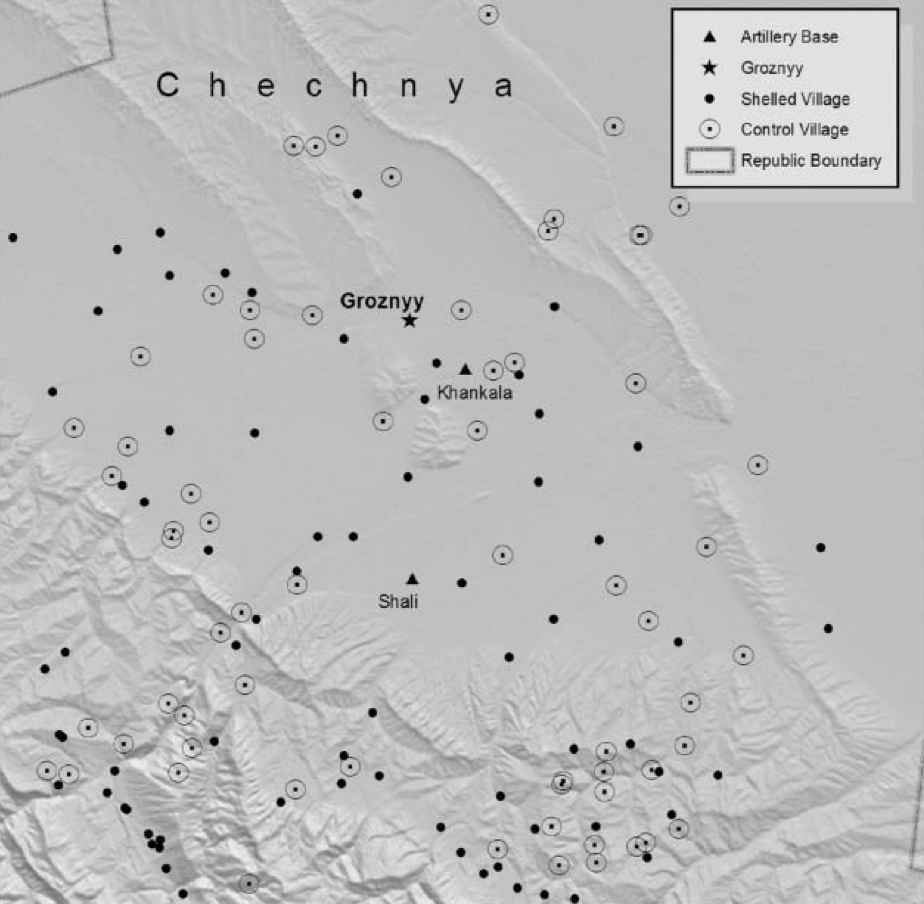
\includegraphics[width = .8 \linewidth]{images/lyall_map.png}
%\end{figure}
%
%\end{frame}
%
%\begin{frame}{Identification Strategy: Doctrine and Drunks}
%
%\textbf{``Harassment and Interdiction'' Doctrine}: ``barrages at random
%intervals and of varying duration on random days'' \pause \bigskip
%
%\textbf{Drunks}: ``As one Russian commander put it, solders `get drunk
%as pigs, lob a few shells, claim combat pay and get drunk again'.''"
%
%\end{frame}
%
%\begin{frame}{Balance Checks}
%
%\begin{figure}[ht] \centering
%    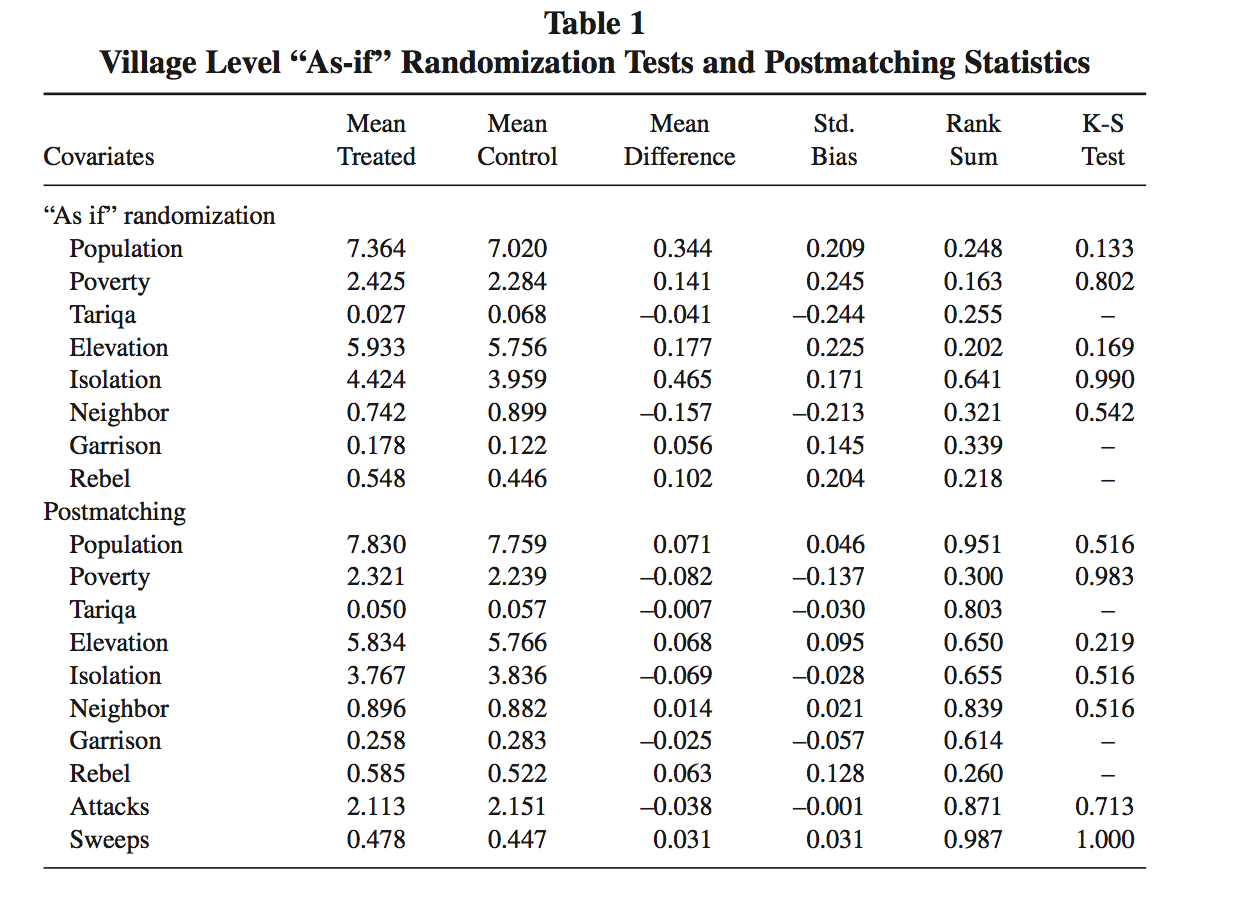
\includegraphics[width = .99 \linewidth]{images/lyall_balance.png}
%\end{figure}
%
%\end{frame}

%\begin{frame}{Gilligan and Sargenti (2008)}
%
%\begin{figure}[ht] \centering
%    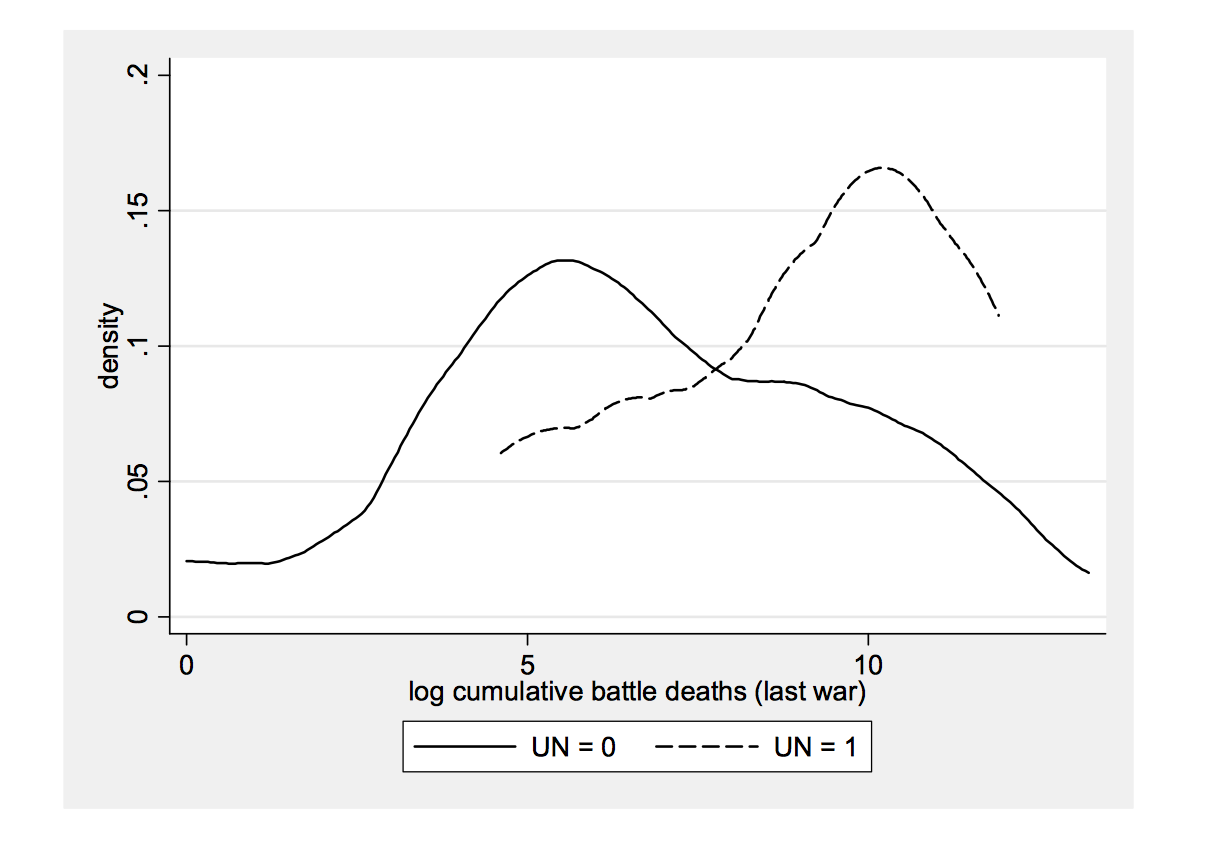
\includegraphics[width = .99 \linewidth]{images/gilligan_sargenti_balance.png}
%\end{figure}
%
%\end{frame}

%\begin{frame}{Gilligan and Sargenti (2008)}
%
%\begin{figure}[ht] \centering
%    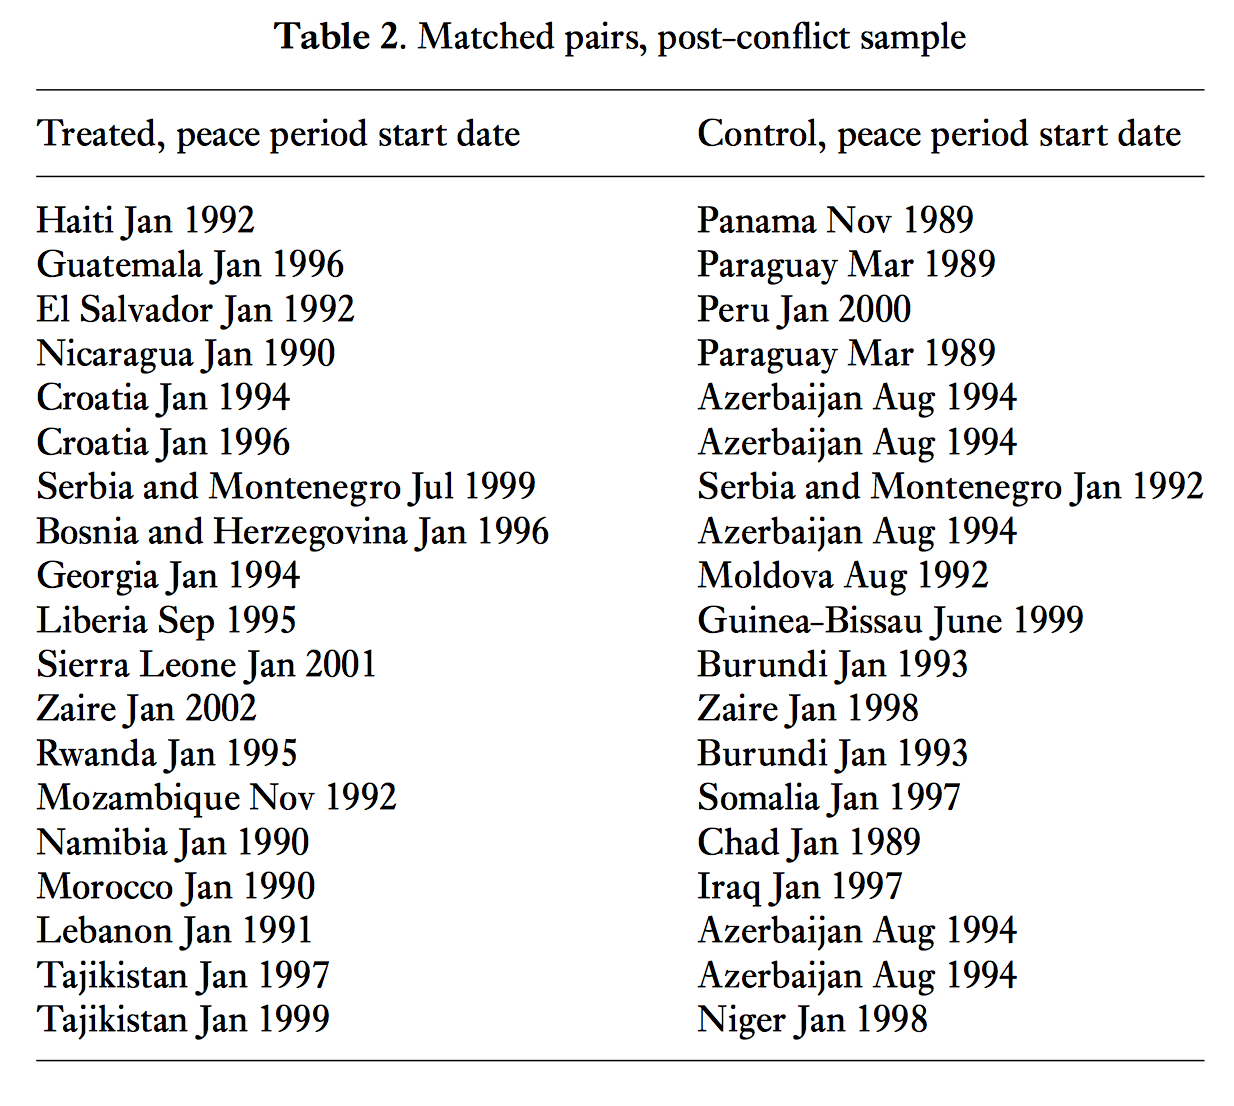
\includegraphics[width = .99 \linewidth]{images/gilligan_sargenti_matched_pairs.png}
%\end{figure}
%
%\end{frame}


\begin{frame}{ATT Estimation by Matching}
\small
\begin{itemize} 
\item<1-> For each treated unit $i$ with covariates $X_i$, you would like to estimate $\tau_i=Y_{1i}-Y_{0i}$. 
\item<2-> For treated units you observe $Y_{1i}$, but where to get $Y_{0i}$? 
\item<3-> \textcolor{Blue}{Matching}: borrow it from control unit with (nearly) the same $X_i$ 
%\begin{align*} 
%\tau(X_i) &= Y_{1i}|X_i]-\E[Y_{0i}|X_i] \\
%&= \E[Y_i|D_i=1, X_i]-\E[Y_i|D_i=0, X_i] \quad \text{ \alert{(Why?)}}
%\end{align*}
%\item<2-> The $Y_{1i}$
%\item<3-> But where to get $Y_i|D_i=0, X_i$?
%\item<4-> Control unit \alert{nearest} to $X_i$? 
%\item<5-> In other words, nearest control unit's outcome is taken as counterfactual for the treated unit's $Y_{0i}$.
\item<4-> So estimator is:
\end{itemize}
\onslide<4-> \[
\widehat{\tau}_{ATT}= \frac{1}{N_1} \sum_{D_i=1}
\big(Y_i - Y_{j(i)}\big)
\] \footnotesize where $Y_{j(i)}$ is the outcome of an untreated observation such that
$X_{j(i)}$ is the \alert{closest} value to $X_i$ among the untreated
observations.\\
\small
\medskip 
\onslide<5-> We can also use the average of $M$ closest matches: \[
\widehat{\tau}_{ATT}= \frac{1}{N_1} \sum_{D_i=1} \left\{ Y_i -
\left(\frac{1}{M}\sum_{m=1}^M Y_{j_m(i)},\right)\right\}
\] 

\onslide<6-> Does SOO assumption guarantee that this gets you the $ATT$?
\end{frame}

\begin{frame}{Matching: Example with a Single $X$}
\begin{tabular}{c|c|c|c|c}
 & Potential Outcome & Potential Outcome &   & \\
unit &under Treatment  & under Control &   &  \\

\hline
   i  & $Y_{1i}$  & $Y_{0i}$ &    $D_i$ &  $X_i$ \\
\hline
         1 & \multicolumn{ 1}{c|}{6} & \multicolumn{ 1}{c|}{\textcolor{red}{?}} &                    1 &          3 \\
         2 & \multicolumn{ 1}{c|}{1} & \multicolumn{ 1}{c|}{\textcolor{red}{?}} &                    1 &          1 \\
         3 & \multicolumn{ 1}{c|}{0} & \multicolumn{ 1}{c|}{\textcolor{red}{?}} &                    1 &          10 \\
\hline
         4 & \multicolumn{ 1}{c|}{} & \multicolumn{1}{c|}{0} &                    0 &          2 \\
         5 & \multicolumn{ 1}{c|}{} & \multicolumn{1}{c|}{9} &                    0 &          3 \\
         6 & \multicolumn{ 1}{c|}{} & \multicolumn{1}{c|}{1} &                    0 &          -2 \\
         7 & \multicolumn{ 1}{c|}{} & \multicolumn{1}{c|}{1} &                    0 &          -4 \\
         \hline
\end{tabular}

What is
$\widehat{\tau}_{ATT}= \frac{1}{N_1} \sum_{D_i=1} \big(Y_i - Y_{j(i)}\big)$?
\end{frame}

\begin{frame}{Matching: Example with a Single $X$}

\begin{tabular}{c|c|c|c|c}
 &Potential Outcome & Potential Outcome &   & \\
unit &under Treatment  & under Control &   &  \\

\hline
   i  & $Y_{1i}$  & $Y_{0i}$ &    $D_i$ &  $X_i$ \\
\hline
         1 & \multicolumn{ 1}{c|}{6} & \multicolumn{ 1}{c|}{\textcolor{blue}{9}} &                    1 &          \textcolor{blue}{3} \\
         2 & \multicolumn{ 1}{c|}{1} & \multicolumn{ 1}{c|}{\textcolor{cyan}{0}} &                    1 &          \textcolor{cyan}{1} \\
         3 & \multicolumn{ 1}{c|}{0} & \multicolumn{ 1}{c|}{\textcolor{blue}{9}} &                    1 &          \textcolor{blue}{10} \\
\hline
         4 & \multicolumn{ 1}{c|}{} & \multicolumn{1}{c|}{\textcolor{cyan}{0}} &                    0 &          \textcolor{cyan}{2} \\
         5 & \multicolumn{ 1}{c|}{} & \multicolumn{1}{c|}{\textcolor{blue}{9}} &                    0 &          \textcolor{blue}{3} \\
         6 & \multicolumn{ 1}{c|}{} & \multicolumn{1}{c|}{1} &                    0 &          -2 \\
         7 & \multicolumn{ 1}{c|}{} & \multicolumn{1}{c|}{1} &                    0 &          -4 \\
         \hline
\end{tabular}

What is
$\widehat{\tau}_{ATT}= \frac{1}{N_1} \sum_{D_i=1} \big(Y_i - Y_{j(i)}\big)$?
\pause

$\widehat{\tau}_{ATT}=1/3\cdot(6-\textcolor{blue}{9})+1/3\cdot(1-\textcolor{cyan}{0})+1/3\cdot(0-\textcolor{blue}{9})=-3.7$

\end{frame}
\subsection{Measuring Distance}
\begin{frame}{Common Distance Metrics}
\footnotesize
\onslide<1-> What do we mean by ``closeness'' in $X$ when it is multi-dimensional? \\
\medskip
Covariate vectors for $i,j$: $X_i=[X_i^{(1)},X_i^{(2)},...,X_i^{(k)}]^{\top}$ and 
$X_j=[X_j^{(1)},X_j^{(2)},...,X_j^{(k)}]^{\top}$ \\
\bigskip
\onslide<2-> Some common options:
\begin{enumerate}
\item<2-> Euclidean distance:
\begin{align*}
||X_i-X_j|| &= \sqrt {(X_i-X_j)^{\top}(X_i-X_j)} \\
&= [(X_i^{(1)}-X_j^{(1)})^2+...+(X_i^{(P)}-X_j^{(P)})^2 ]^{\frac{1}{2}}
\end{align*}

\item<3-> ``StataD'' (\texttt{nnmatch})/default in \texttt{Match()} for \texttt{R}: rescaled Euclidean
\[
StataD(X_i,X_j)=\sqrt{(X_i-X_j)^{\top}diag(\Sigma_X^{-1})(X_i-X_j)}
\]
where $\Sigma$ is the Variance-Covariance-Matrix. Invariant to rescaling of $X$\\
\end{enumerate}

\end{frame}

\begin{frame}{Common Distance Metrics}
\small
\begin{enumerate}
  \setcounter{enumi}{2}
\item<1-> Mahalanobis distance: 
\[
MD(X_i,X_j)=\sqrt{(X_i-X_j)^{\top}\Sigma^{-1}(X_i-X_j)}
\] where $\Sigma$ is the Variance-Covariance-Matrix. Invariant to rescaling and rotations of $X$\\
\bigskip
\item<2-> GeneticD (\texttt{GenMatch}):
\[
GeneticD(X_i,X_j) = \sqrt{(X_i - X_j)^{\top}(S^{-1/2})^{\top}\, W\, S^{-1/2} (X_i - X_j)}
\] where $W$ is a $(P \times P)$ positive definite weight matrix with zeros in off-diagonals, controlling ``variable  importance''
\end{enumerate}

\end{frame}

\begin{frame}{Mahalanobis Distance: Example}

\begin{table}[!h]
 \begin{center}
 \begin{tabular}{ccc}
\multicolumn{1}{l}{}&
\multicolumn{1}{c}{$X_1$}&
\multicolumn{1}{c}{$X_2$}
\\ \hline
Treated &$0$&$  0$\\
Control A &$ 2$&$2$\\
Control B &$ 1.8$&$0$\\
\hline
\end{tabular}
\end{center}
\end{table}

$X_T=\left(\begin{array}{cc} 0 & 0 \\ \end{array}      \right)^{\top} $
$\quad X_A=\left( \begin{array}{cc} 2 & 2 \\                 \end{array} \right)^{\top} $
$\quad X_B=\left( \begin{array}{cc} 1.8 &  0 \\                 \end{array} \right)^{\top} $\\\bigskip

$\quad \Sigma=\left( \begin{array}{ccc}                   & X^{(1)} & X^{(2)} \\                  
X^{(1)} & 1 &  .9 \\                  
X^{(2)} & .9 & 1\\  \end{array}              \right)$\\\bigskip

Which control is closer?

\end{frame}

\begin{frame}{Mahalanobis Distance}
\scriptsize
$X_T=\left(\begin{array}{cc} 0 & 0 \\\end{array}    \right)^{\top}, $
$\,\, X_A=\left(                 \begin{array}{cc}                   2 &  2 \\                 \end{array}               \right)^{\top}, $
$\,\, X_B=\left(                 \begin{array}{cc}                   1.8 &  0 \\                 \end{array}               \right)^{\top}, $
$\,\,\Sigma=\left(                \begin{array}{ccc}           & X^{(1)} & X^{(2)} \\                  X^{(1)} & 1 &  .9 \\                  X^{(2)} & .9 & 1\\                \end{array}              \right)$

\begin{align*}
MD(X_A,X_{T}) &= \sqrt{
(X_A-X_T)^{\top} \Sigma^{-1}(X_A-X_T)}\\
 &=  \sqrt{
[\left(
       \begin{array}{cc}
         2 & 2 \\
       \end{array}
     \right)-\left(
                \begin{array}{cc}
                  0 &  0 \\
                \end{array}
              \right)] \left(
               \begin{array}{cc}
                  1 &  .9 \\
                   .9 & 1 \\
               \end{array}
             \right)^{-1} [\left(
       \begin{array}{cc}
         2 & 2 \\
       \end{array}
     \right)-\left(
                \begin{array}{cc}
                    0 &  0 \\
                \end{array}
              \right)]^{\top}}\\
& =  \sqrt{
\left[
       \begin{array}{cc}
         2 &  2 \\
       \end{array}
     \right] \left(
               \begin{array}{cc}
                   5.2 &  -4.7 \\
                   -4.7 & 5.2 \\
               \end{array}
             \right)\left[
       \begin{array}{cc}
         2 &  2 \\
       \end{array}
     \right]^{\top}}\\
 &= 4.2\\
MD(X_B,X_{T}) &=  \sqrt{
\left[
       \begin{array}{cc}
         1.8 &  0 \\
       \end{array}
     \right] \left(
               \begin{array}{cc}
                   5.2 &  -4.7 \\
                   -4.7 & 5.2 \\
               \end{array}
             \right)\left[
       \begin{array}{cc}
          1.8 &  0 \\
       \end{array}
     \right]^{\top}}\\
 &= 17\\
\end{align*}
%With $StataD(X_A,X_T)=\sqrt{(X_i-X_T)^{\top} diag(\Sigma_X^{-1})(X_i-X_T)}$ we find $StataD(X_A,X_T)=84$ and $StataD(X_B,X_T)=17$ since correlation is ignored.
\end{frame}

\begin{frame}{Mahalanobis Distance}
\vspace{-.2in}
\begin{figure}[ht] \centering
    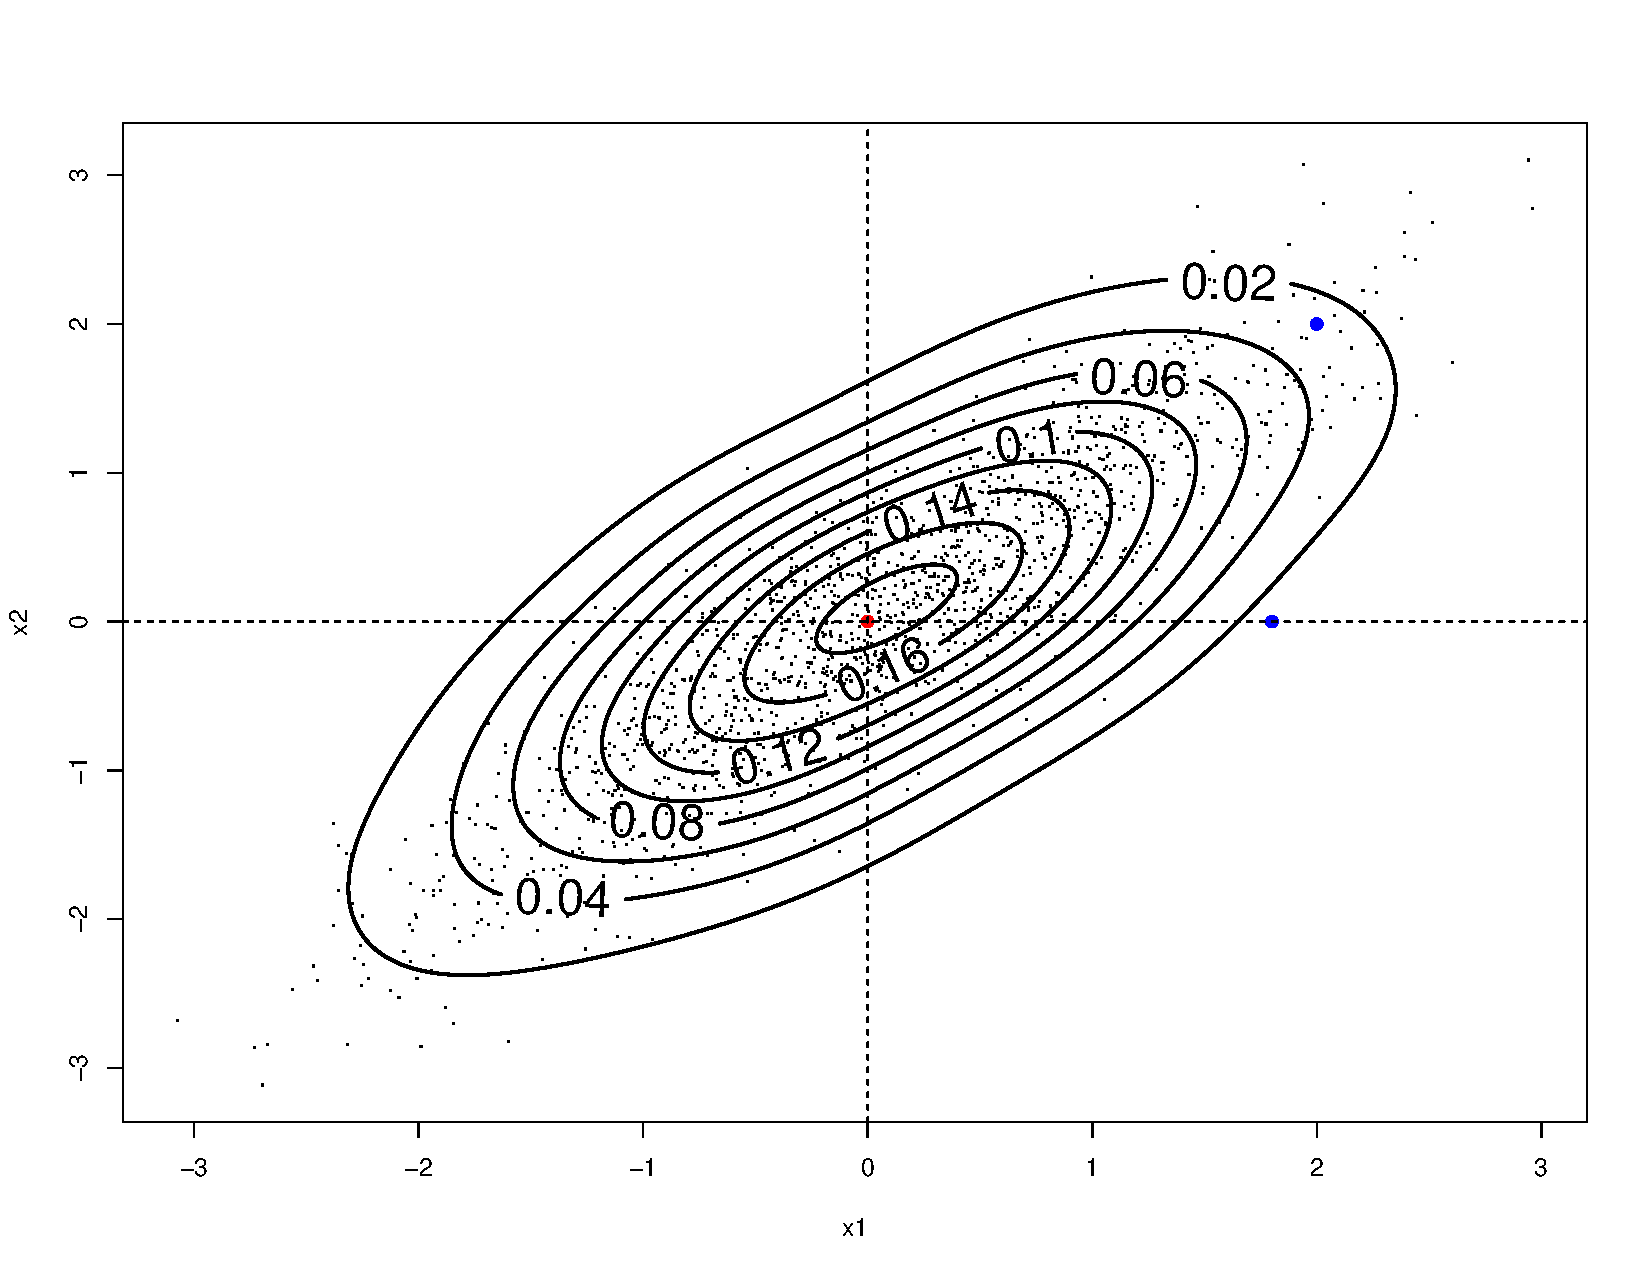
\includegraphics[width = .9 \linewidth]{images/Maha1.pdf}
\end{figure}
\end{frame}

%\begin{frame}{Normalized Euclidean Distance}
%\vspace{-.2in}
%\begin{figure}[ht] \centering
%    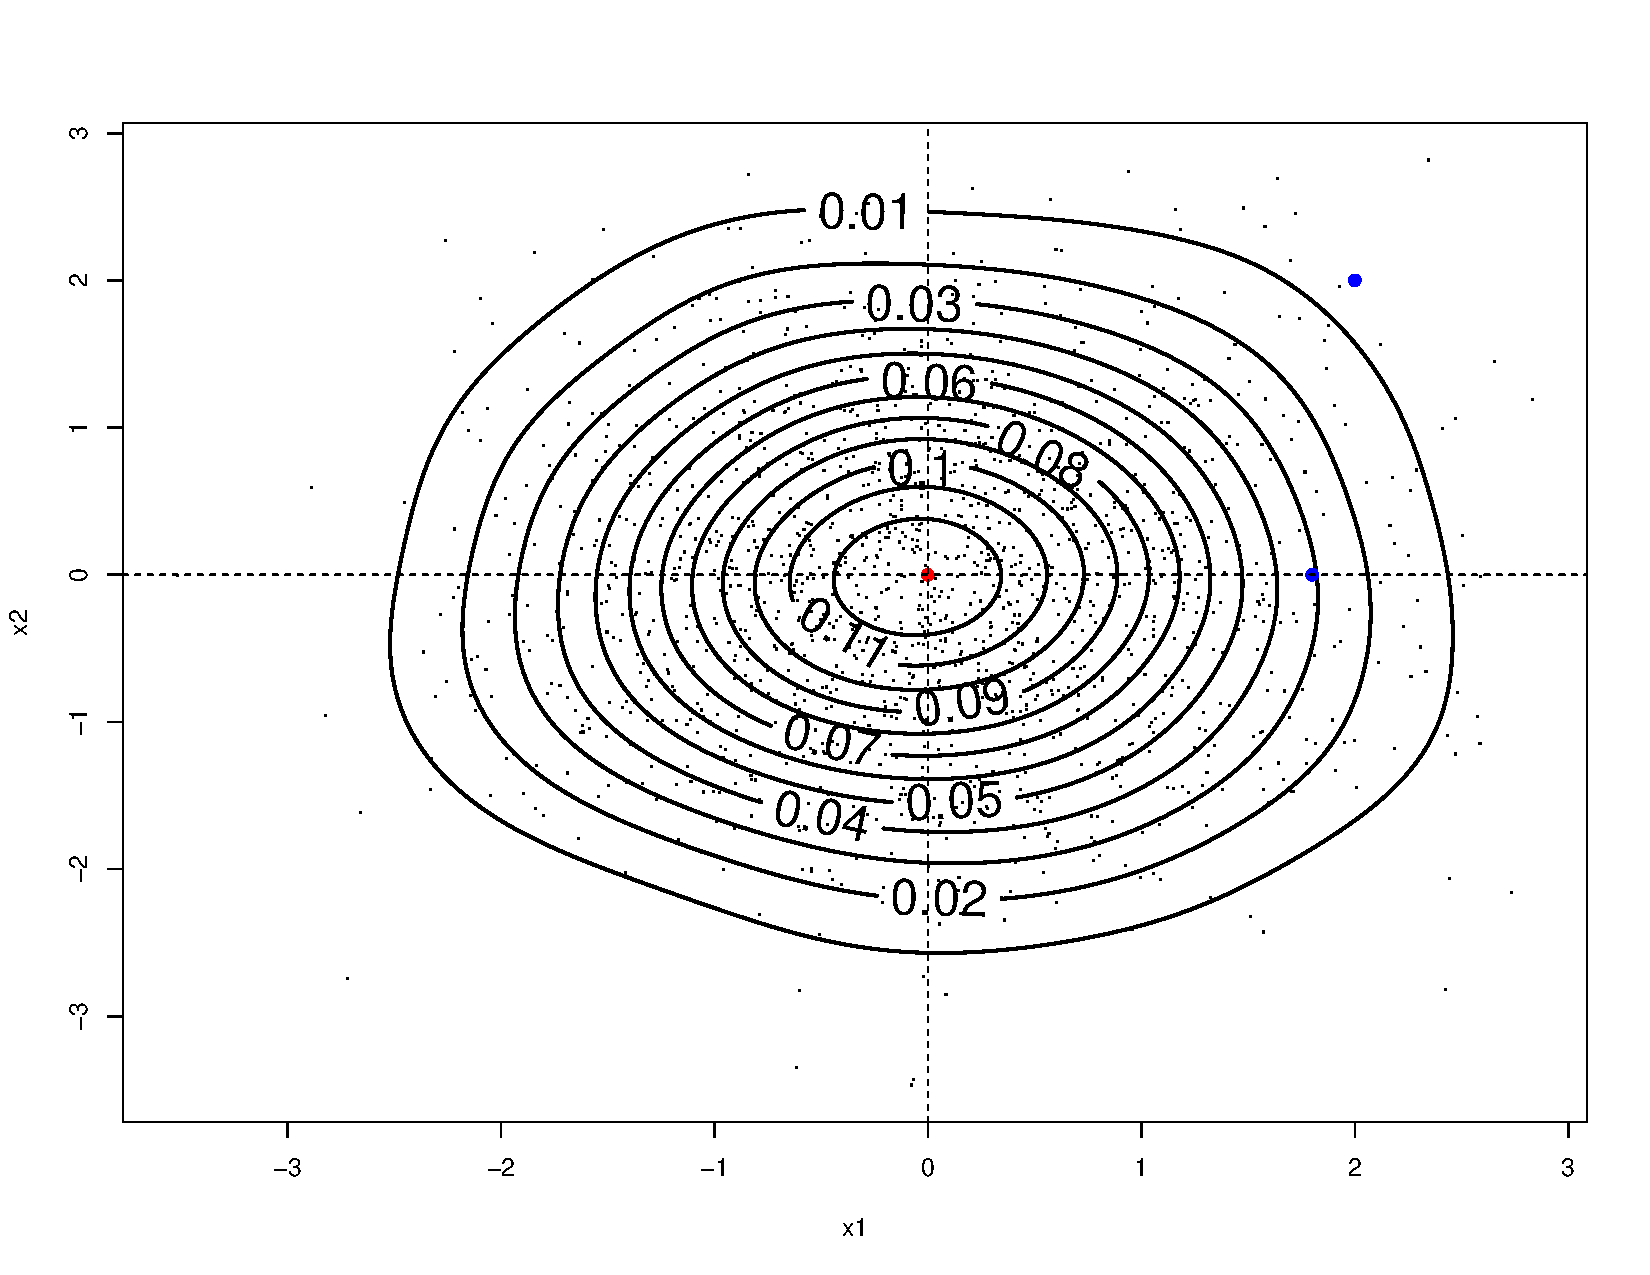
\includegraphics[width = .9 \linewidth]{images/Maha2.pdf}
%\end{figure}
%
%\end{frame}

%\begin{frame}{Genmatch}
%
%\begin{figure}[ht] \centering
%    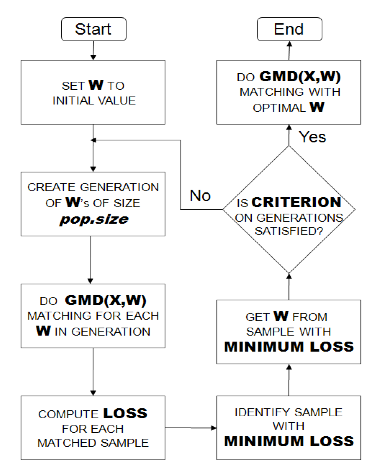
\includegraphics[width = .5 \linewidth]{images/genmatch_flow_chart.png}
%\end{figure}
%
%\end{frame}

%\begin{frame}{Genmatch}
%
%\begin{figure}[ht] \centering
%    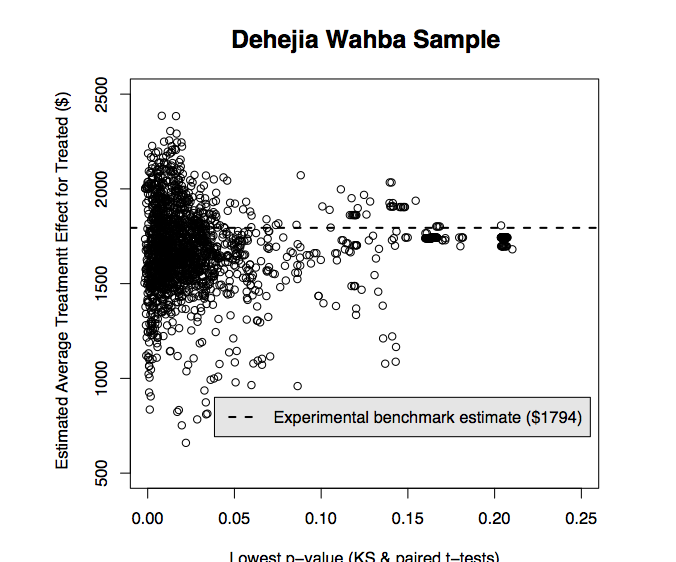
\includegraphics[width = .8 \linewidth]{images/genmatch.png}
%\end{figure}
%
%\end{frame}

\begin{frame}{Local Methods and the Curse of Dimensionality}
\small
Problem: the volume increases \alert{exponentially} in dim(X).
%\vspace{-.4cm}
\begin{figure}[ht] \centering
    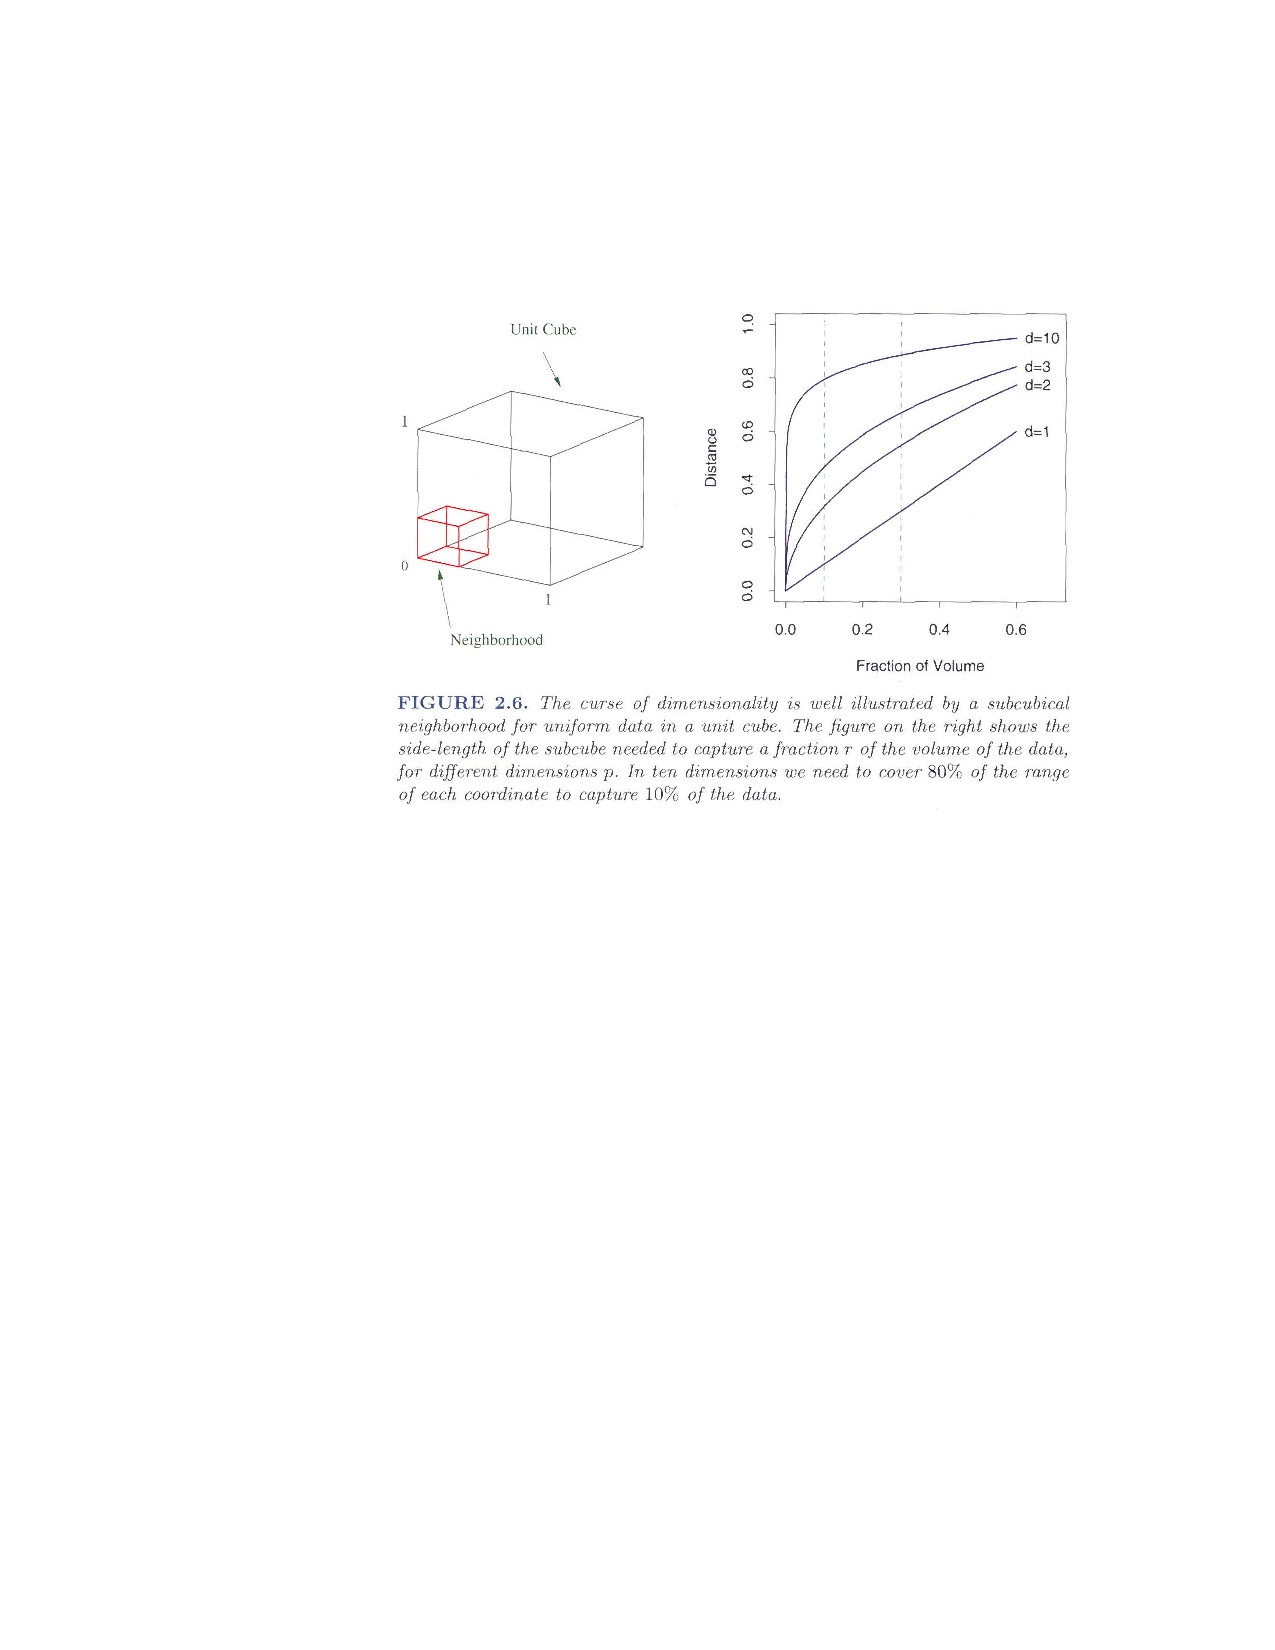
\includegraphics[width = .6 \linewidth]{images/curse_dimensionality1.pdf}
\end{figure}

\end{frame}

%\begin{frame}{Local Methods and the Curse of Dimensionality}
%\begin{figure}[ht] \centering
%    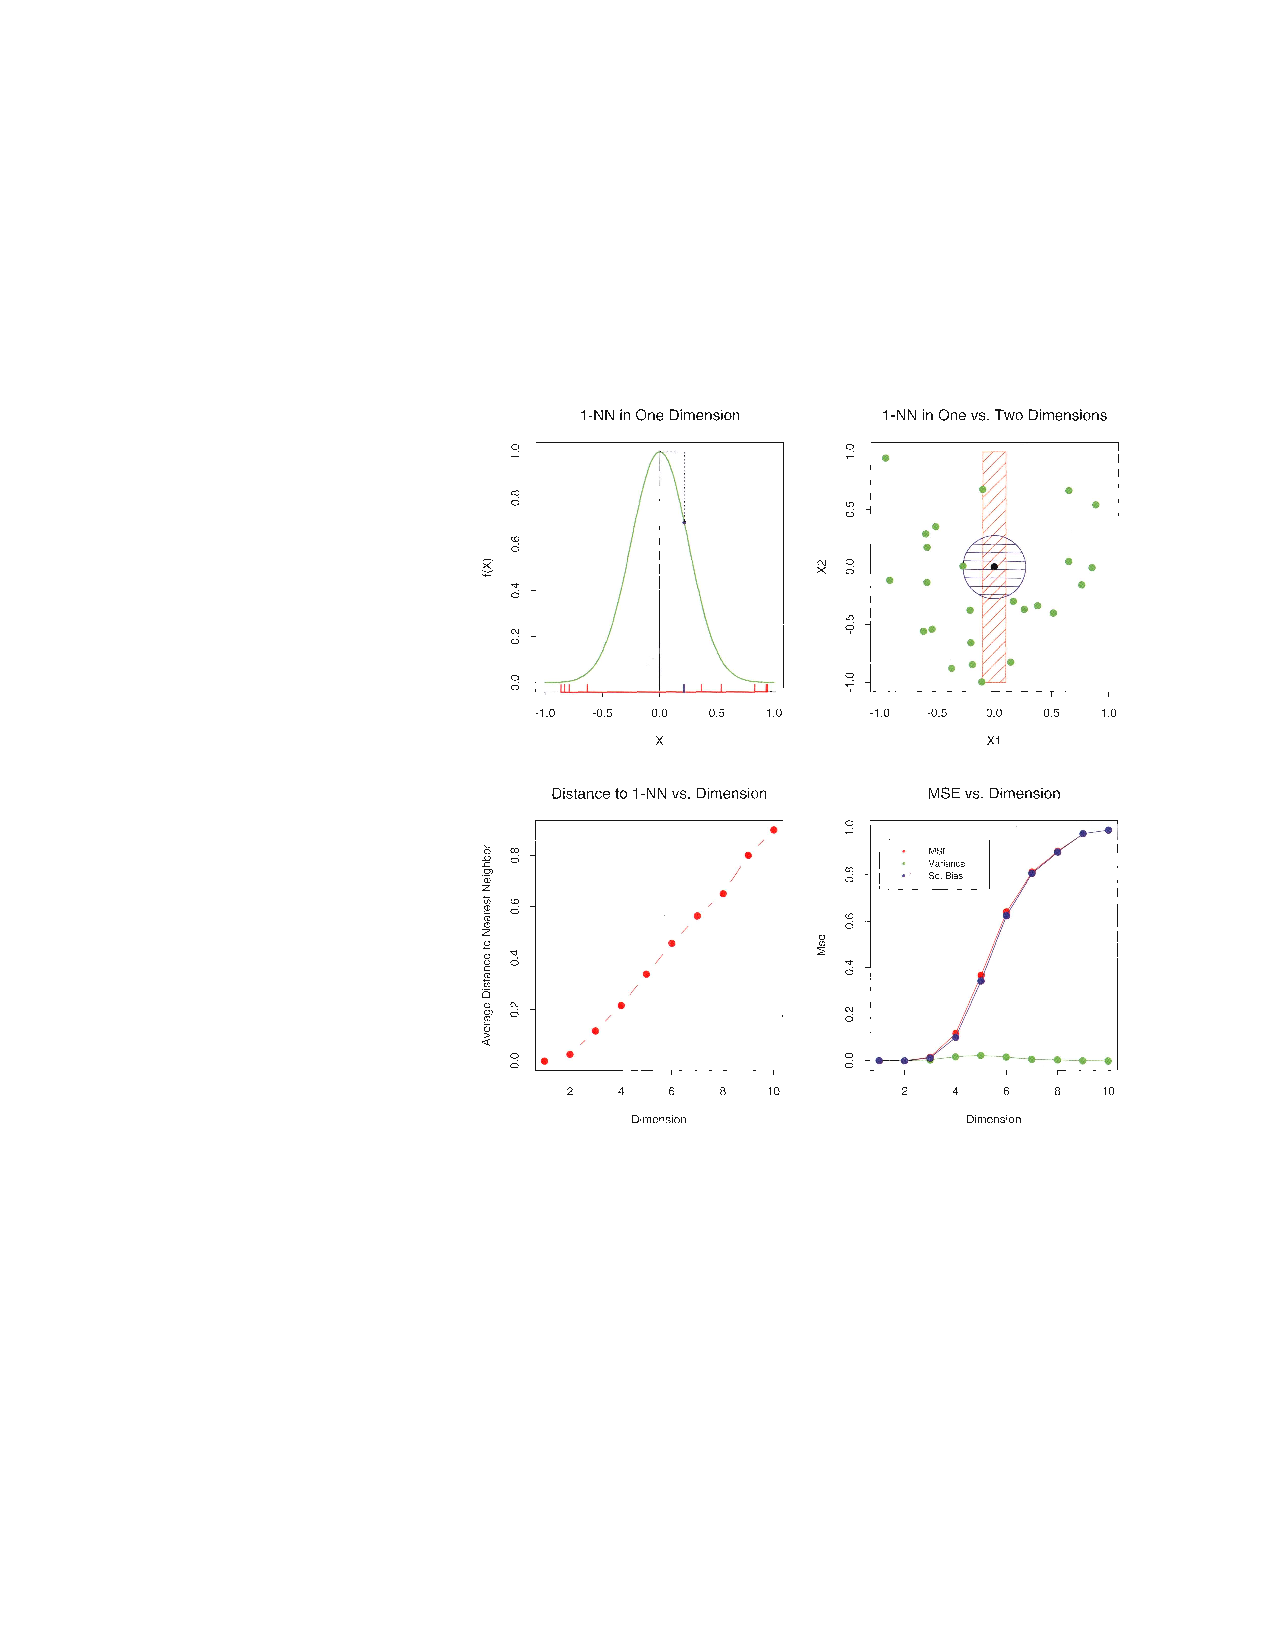
\includegraphics[width = .5 \linewidth]{images/curse_dimensionality2.pdf}
%\end{figure}
%\end{frame}

\begin{frame}{Matching with Bias Correction}
\small
\onslide<1-> Weakness of matching: \alert{discrepancy}=$||X_i-X_{j(1)}||_d>0$ \\
\bigskip
\onslide<2-> With multiple continuous variables, this becomes problematic
\begin{itemize}
\footnotesize
\item  if $X$ predicts treatment, then this discrepancy is not just random noise \\
\item<3-> does not average away quickly: not $\sqrt{N}$ consistent (Abadie and Imbens, 2005)
\end{itemize}
\small
\bigskip
\onslide<4-> Compromise: adjust for discrepancy:
\begin{itemize}
\item On average, $Y_{0j}$ differs from $Y_{0i}$ by $\E[Y_0|X_i]-\E[Y_0|X_{j(i)}]$
\item Consider population regression function $\mu_0(X)=\E[Y_0|X]$
\item Let's estimate $\hat{\mu}_0$ by OLS regression of $Y$ on $X$ among controls \[ \hat{\mu}_0(X)=\beta_0+\beta_1 X \] 
\end{itemize}
\end{frame}

\begin{frame}{Matching with Bias Correction}
\onslide<1-> So subtract off estimated discrepancy on $Y_0$ from each pair (Abadie \& Imbens, 2005)
\[\tilde{\tau}_{ATT}= \frac{1}{N_1} \sum_{D_i=1}
((Y_i - Y_{j(i)}) -(\widehat\mu_0(X_i)-\widehat\mu_0(X_{j(i)})),
\] 

\begin{itemize}
\item these ``bias-corrected'' matching estimators are an improvement even if $\hat{\mu_0}$ is misspecified
\item the large sample distribution of this estimator (for the case of matching with replacement) is roughly normal. 
\end{itemize}
\bigskip
In R: \texttt{Match(Y,Tr, X,BiasAdjust = TRUE)}

\end{frame}

\begin{frame}{Bias Adjustment with Matched Data}
\begin{centering}
\begin{tabular}{c|c|c|c|c}
 &Potential Outcome & Potential Outcome &   & \\
unit &under Treatment  & under Control &   &  \\

\hline
   i  & $Y_{1i}$  & $Y_{0i}$ &    $D_i$ &  $X_i$ \\
\hline
         1 & \multicolumn{ 1}{c|}{6} & \multicolumn{ 1}{c|}{\textcolor{red}{?}} &                    1 &          3 \\
         2 & \multicolumn{ 1}{c|}{1} & \multicolumn{ 1}{c|}{\textcolor{red}{?}} &                    1 &          1 \\
         3 & \multicolumn{ 1}{c|}{0} & \multicolumn{ 1}{c|}{\textcolor{red}{?}} &                    1 &          10 \\
\hline
         4 & \multicolumn{ 1}{c|}{} & \multicolumn{1}{c|}{0} &                    0 &          2 \\
         5 & \multicolumn{ 1}{c|}{} & \multicolumn{1}{c|}{9} &                    0 &          3 \\
         6 & \multicolumn{ 1}{c|}{} & \multicolumn{1}{c|}{1} &                    0 &          8 \\
         \hline
\end{tabular}
\end{centering} \\
\bigskip
What is
$\tilde\tau_{ATT}= \frac{1}{N_1}\sum_{D_i=1} \Big((Y_i-Y_{j(i)})- (\widehat\mu_0(X_i)-\widehat\mu_0(X_{j(i)})) \Big)$?

\end{frame}

\begin{frame}{Bias Adjustment with Matched Data}
\footnotesize 
\begin{tabular}{c|c|c|c|c}
 &Potential Outcome & Potential Outcome &   & \\
unit &under Treatment  & under Control &   &  \\
\hline
   i  & $Y_{1i}$  & $Y_{0i}$ &    $D_i$ &  $X_i$ \\
\hline
         1 & \multicolumn{ 1}{c|}{6} & \multicolumn{ 1}{c|}{\textcolor{blue}{9}} &                    1 &          3 \\
         2 & \multicolumn{ 1}{c|}{1} & \multicolumn{ 1}{c|}{\textcolor{cyan}{0}} &                    1 &          1 \\
         3 & \multicolumn{ 1}{c|}{0} & \multicolumn{ 1}{c|}{\textcolor{green}{1}} &                    1 &          10 \\
\hline
         4 & \multicolumn{ 1}{c|}{} & \multicolumn{1}{c|}{0} &                    0 &          \textcolor{cyan}{2} \\
         5 & \multicolumn{ 1}{c|}{} & \multicolumn{1}{c|}{9} &                    0 &          \textcolor{blue}{3} \\
         6 & \multicolumn{ 1}{c|}{} & \multicolumn{1}{c|}{1} &                    0 &          \textcolor{green}{8} \\
         \hline
\end{tabular}

What is
$\tilde\tau_{ATT}= \frac{1}{N_1}\sum_{D_i=1} \Big((Y_i-Y_{j(i)})- (\widehat\mu_0(X_i)-\widehat\mu_0(X_{j(i)})) \Big)$?

Estimate $\widehat\mu_0(x)=\beta_0 + \beta_1 x = 5 - .4 x$. \pause Now
plug in:
\vspace{-.1in}
\begin{eqnarray*}
\widehat{\tau}_{ATT} &=&1/3 \{ ((6-\textcolor{blue}{9})-(\widehat\mu_0(3)-\widehat\mu_0(\textcolor{blue}{3})))\\
&+&((1-\textcolor{cyan}{0})-(\widehat\mu_0(1)-\widehat\mu_0(\textcolor{cyan}{2})))\\
&+&((0-\textcolor{green}{1})-
(\widehat\mu_0(10)-\widehat\mu_0(\textcolor{green}{8})))\}\\
&=& \frac{1}{3}[(6-\textcolor{blue}{9}) + 
[(1-\textcolor{cyan}{0})-(4.6-4.2)]+[(0-\textcolor{green}{1})-(1-1.8)]]\\
&=& -0.87  \text{\,\, (rather\, than\, -1)}
\end{eqnarray*}

%(Unadjusted: $ 1/3((6-9) + (1-0) + (0-1) )=-1$)

\end{frame}

%\begin{frame}{Before Matching}
%\vspace{-.3in}
%\begin{figure}[ht] \centering
%    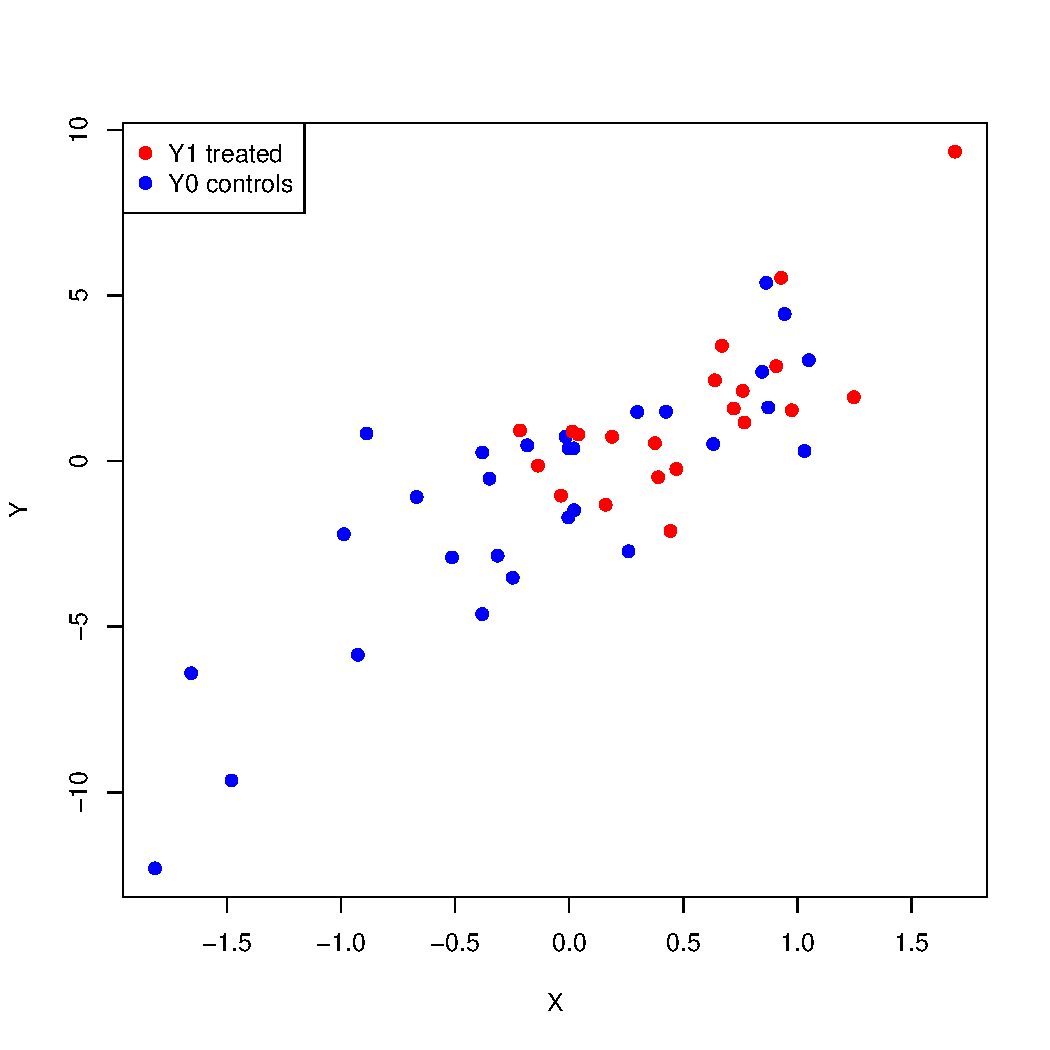
\includegraphics[width = .75 \linewidth]{images/matching_sim1.pdf}
%\end{figure}
%\end{frame}

%\begin{frame}{After Matching}
%\vspace{-.3in}
%\begin{figure}[ht] \centering
%    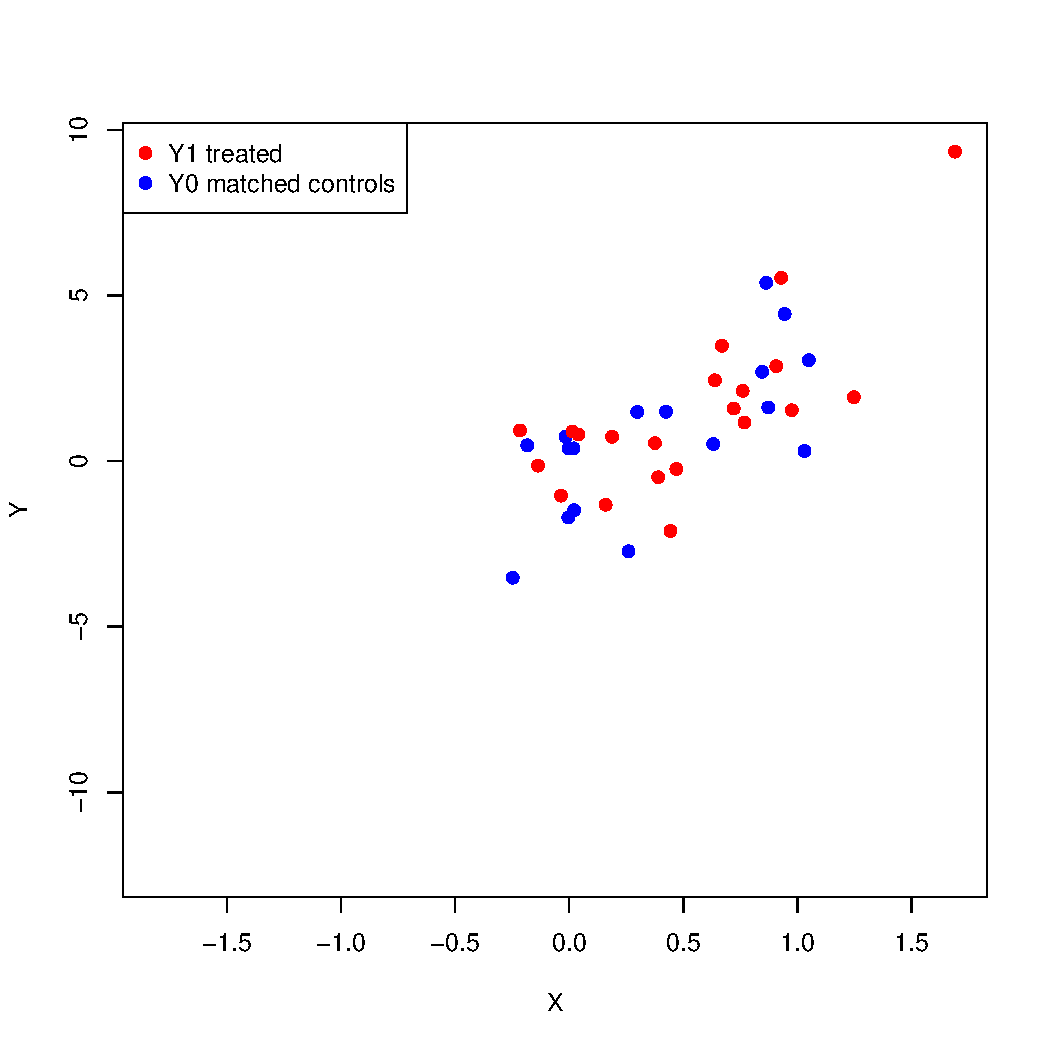
\includegraphics[width = .75 \linewidth]{images/matching_sim2.pdf}
%\end{figure}
%
%\end{frame}
%
%\begin{frame}{After Matching: Imputation Function}
%\vspace{-.3in}
%\begin{figure}[ht] \centering
%    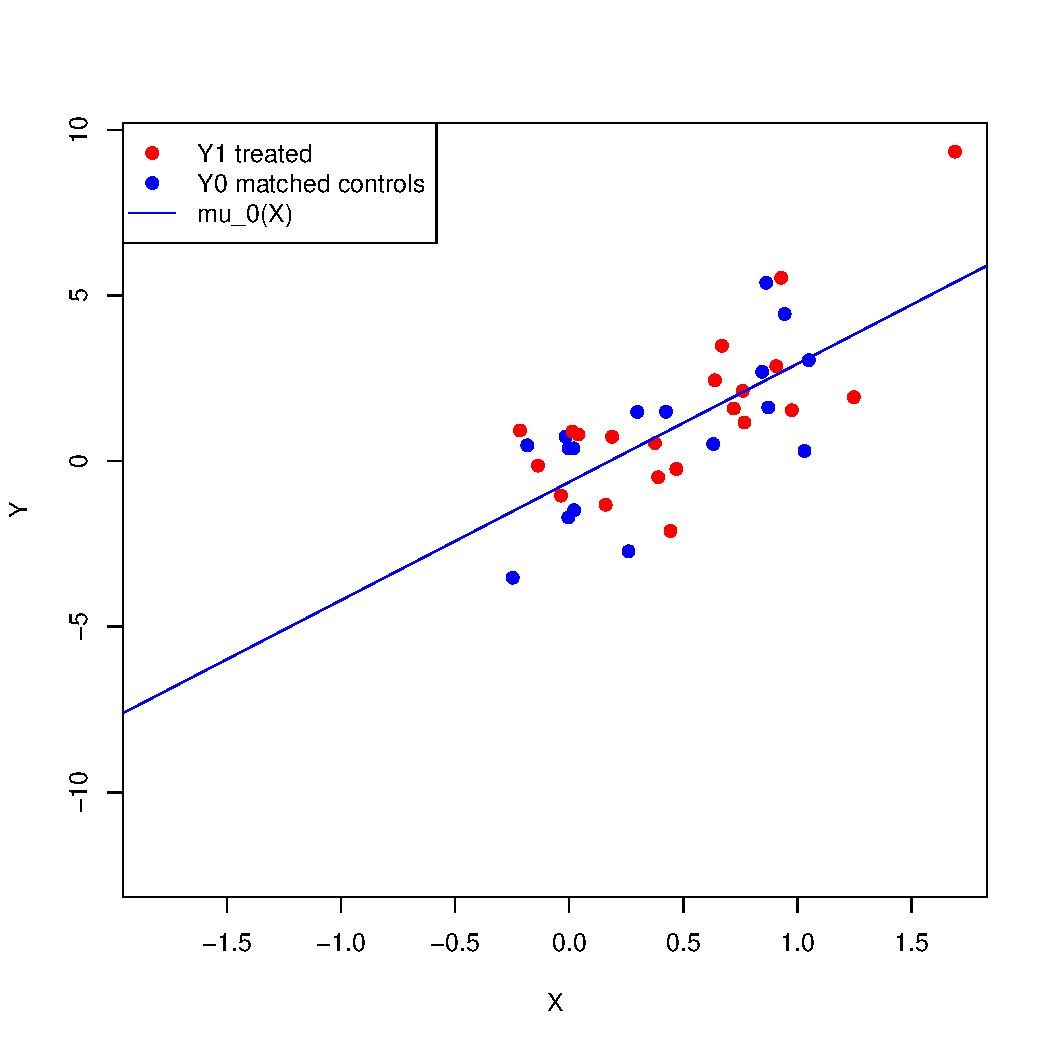
\includegraphics[width = .75 \linewidth]{images/matching_sim3.pdf}
%\end{figure}
%
%\end{frame}
%
%\begin{frame}{After Matching: Imputation of missing $Y_0$}
%\vspace{-.3in}
%\begin{figure}[ht] \centering
%    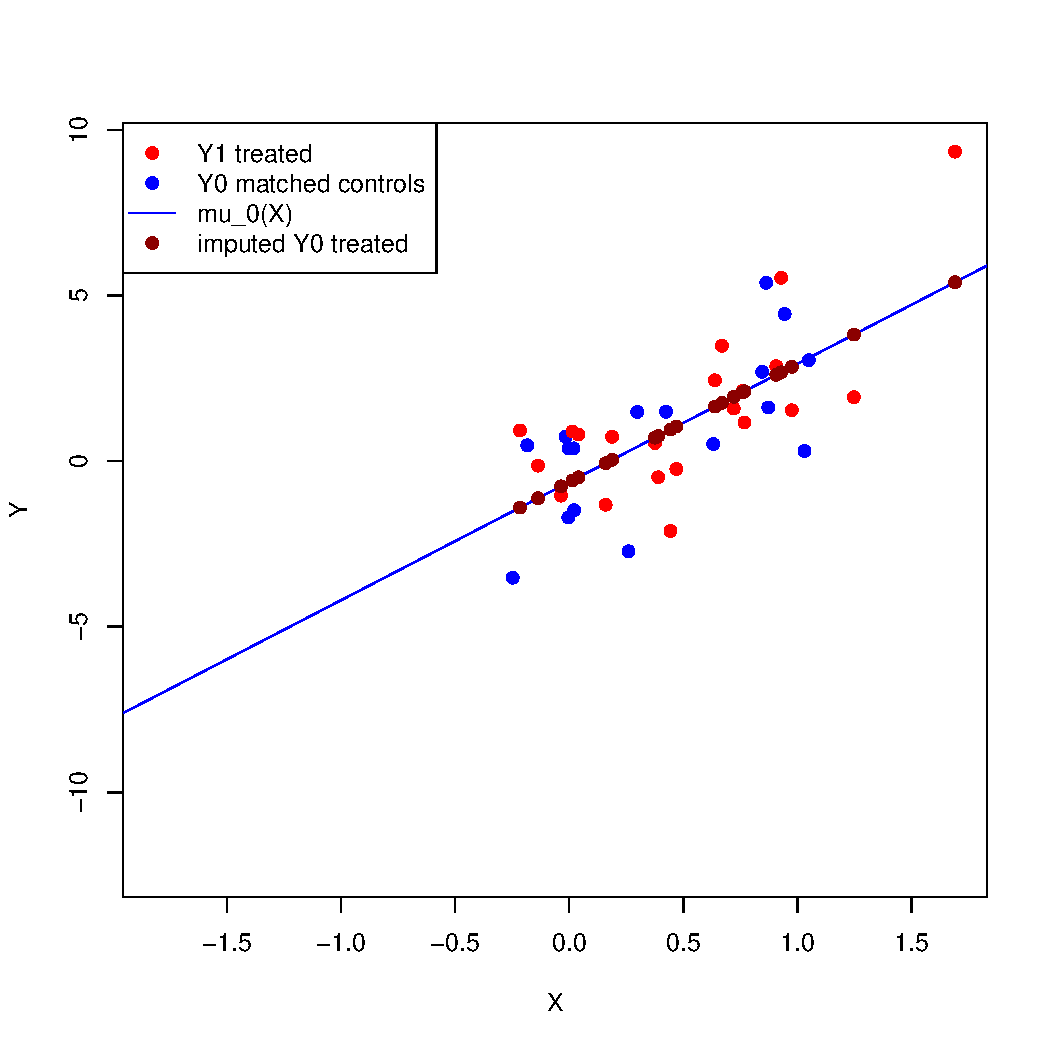
\includegraphics[width = .75 \linewidth]{images/matching_sim4.pdf}
%\end{figure}
%
%\end{frame}
%
%\begin{frame}{After Matching: No Overlap in $Y_0$}
%\vspace{-.3in}
%\begin{figure}[ht] \centering
%    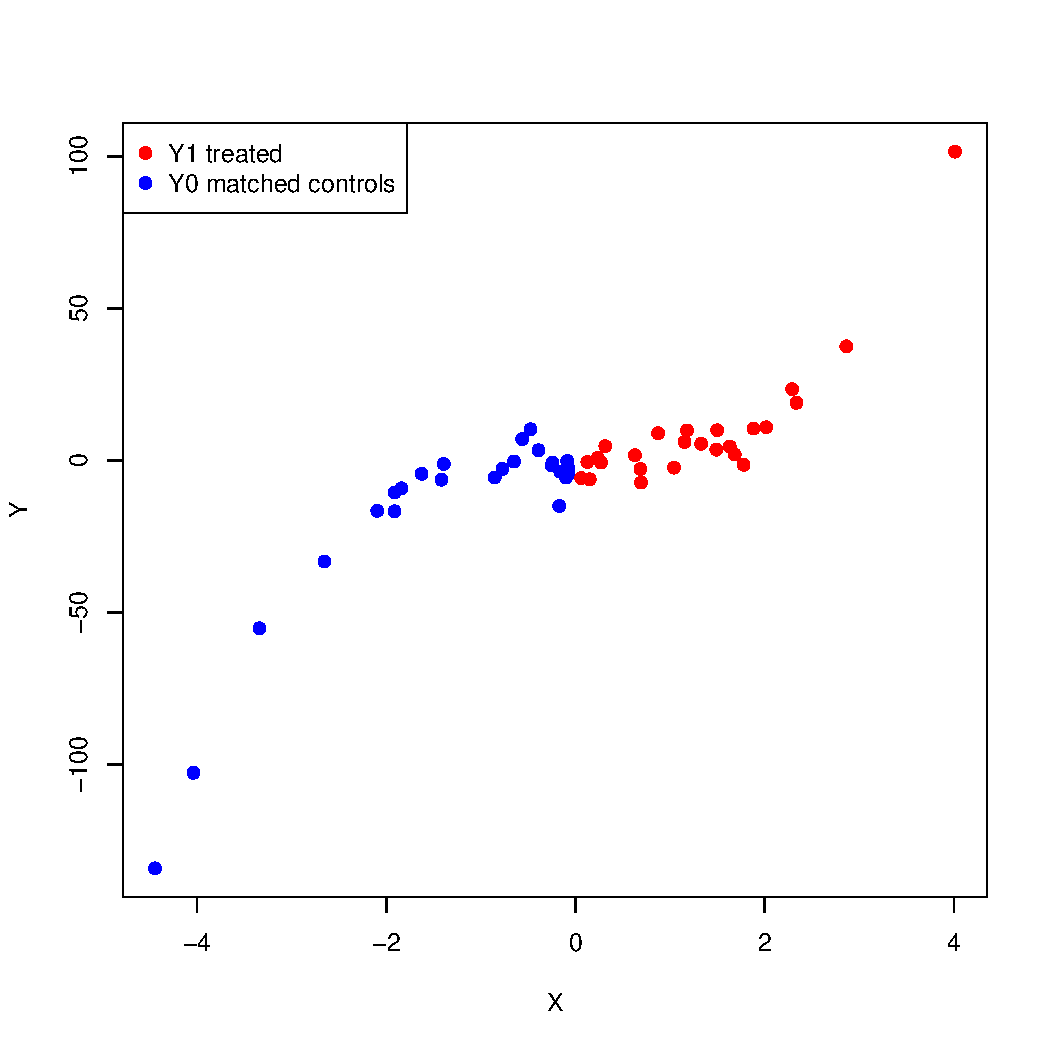
\includegraphics[width = .75 \linewidth]{images/matching_sim5.pdf}
%\end{figure}
%
%\end{frame}
%
%\begin{frame}{After Matching: Imputation of missing $Y_0$}
%\vspace{-.3in}
%\begin{figure}[ht] \centering
%    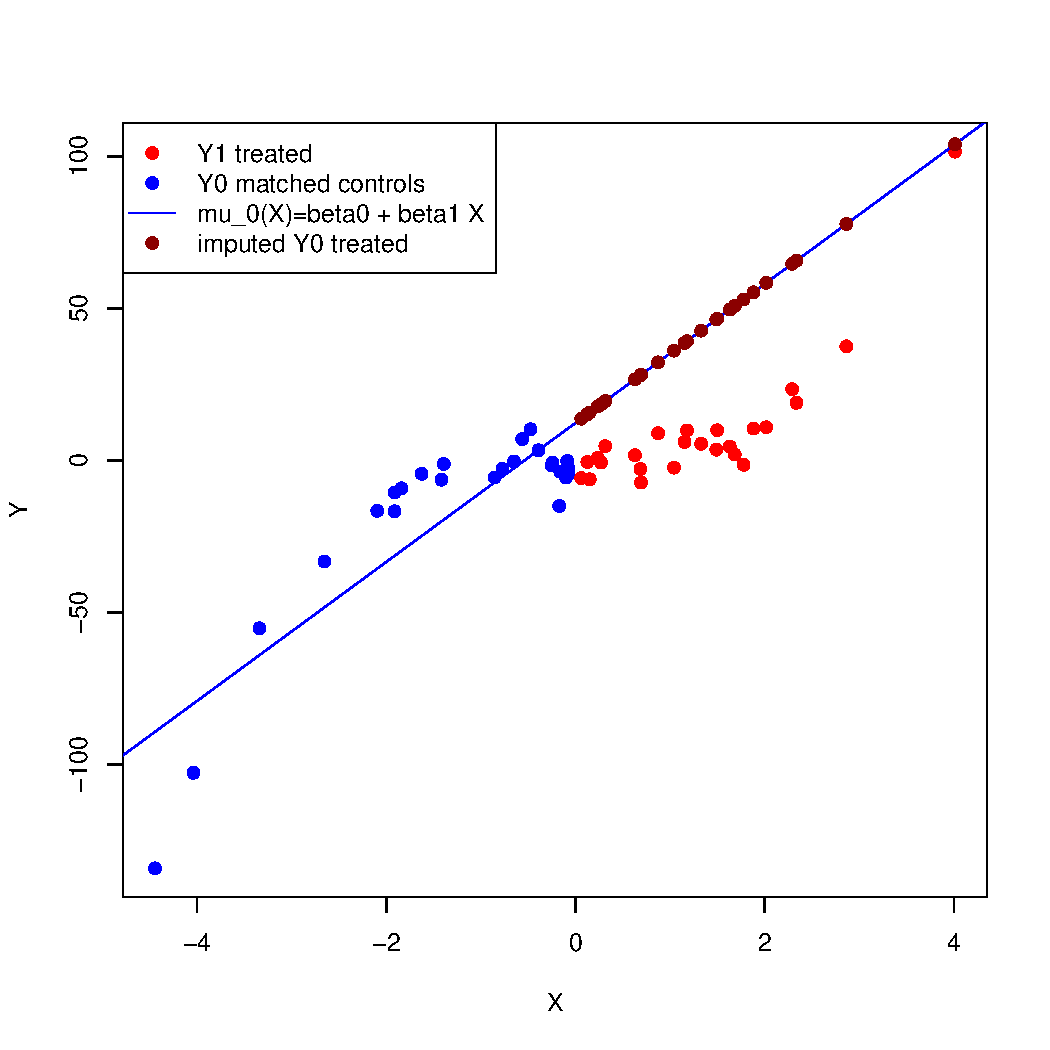
\includegraphics[width = .75 \linewidth]{images/matching_sim6.pdf}
%\end{figure}
%
%\end{frame}
%
%\begin{frame}{After Matching: Imputation of missing $Y_0$}
%\vspace{-.3in}
%\begin{figure}[ht] \centering
%    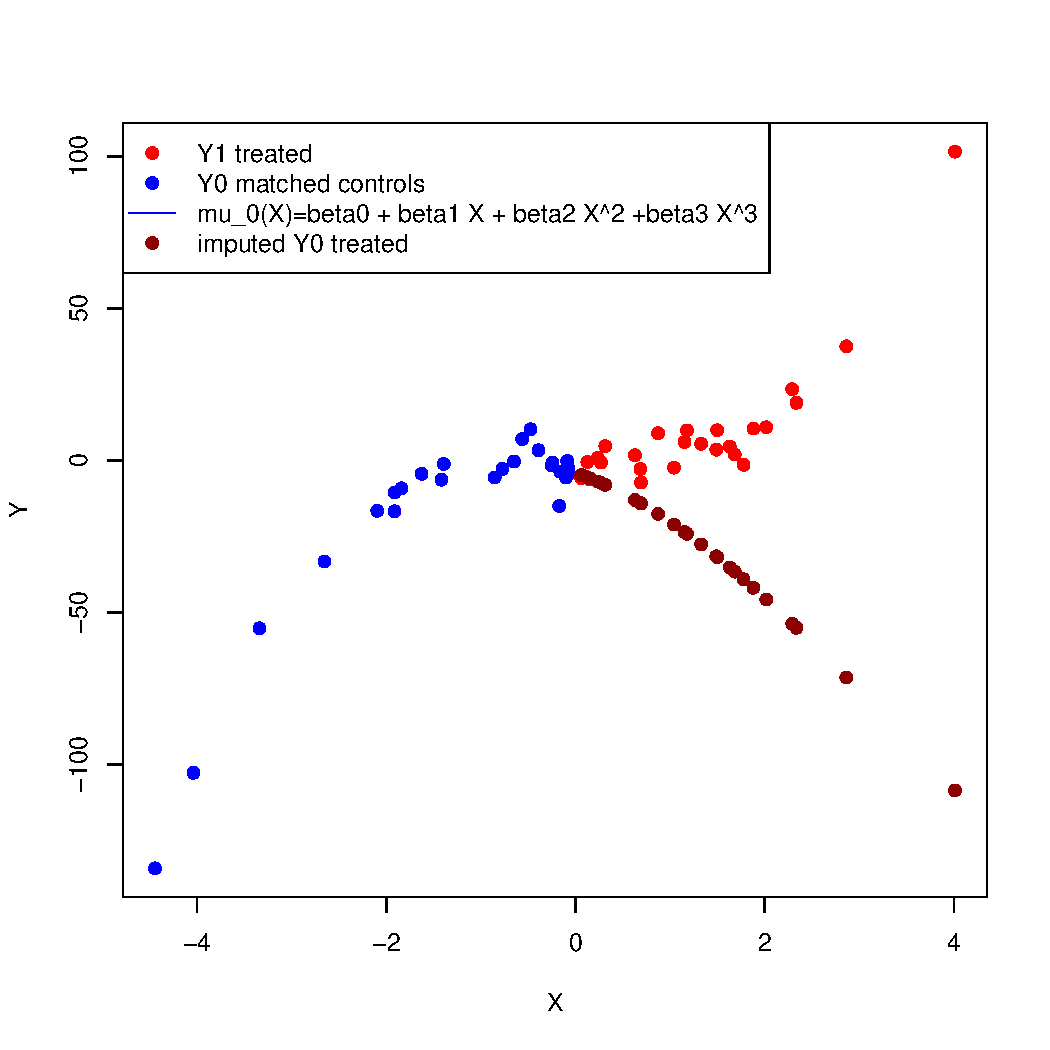
\includegraphics[width = .75 \linewidth]{images/matching_sim7.pdf}
%\end{figure}
%\end{frame}

\subsection{Balance}
\begin{frame}{Checking balance: Theory}
\small
\begin{itemize}
\item<1-> The practice of ``checking balance'' is not necessarily linked to matching, but rose in popularity with it as attention in practice turned to comparability and the analogy to the idea of emulating experiments. \\
\smallskip
\item<2-> Ideally, covariate balance would mean $p(X|D=1) \approx p(X|D=0)$ (at least after some procedure)
\smallskip
\item<3-> In practice, compare various low-dimensional summaries of the data, especially the mean of each $X$.
\smallskip
\small
\item<3-> \alert{Balance tests} are often used (e.g. t-test, F-test, \alert{KS test}) 
\item<4-> Note that hypothesis tests can be misleading in a matching context: you can make everything insignificant by simply dropping lots of observations --- make sure this is not happening (see Hartman \& Hidalgo)
\end{itemize}
\onslide<5-> One workflow:
\begin{itemize}
\item Estimate $\to$ check balance $\to$ re-estimate $\to$ check balance $\to \cdots$ (ad infinitum until you get a good balance)
\item Is this data snooping? No, because blind to $Y$
\end{itemize}
\end{frame}

\begin{frame}
\frametitle{Kolmogorov-Smirnov (KS) Test}
\small
\begin{itemize}
\item<1-> The \alert{KS test} is used to test whether two random variables are sampled from the same distribution
\item<2-> It is nonparametric, meaning it does not work from assumptions about the form of the underlying distribution
\item<3-> Consider $N$ observations of two random variables, $X_0$ and $X_1$. \\
\end{itemize}

{\onslide<4-> \begin{center}
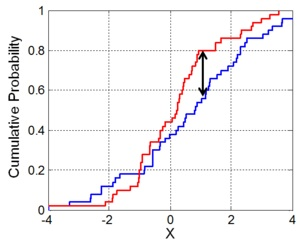
\includegraphics[scale=1.2]{images/KS_Example.jpg}
\end{center}}
\end{frame}


\begin{frame}{Checking balance: Theory}
\small
%\begin{center}
%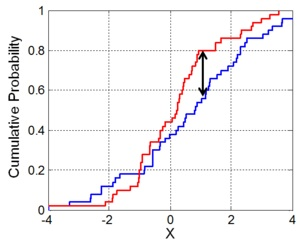
\includegraphics[scale=1]{images/KS_Example.jpg}
%\end{center}
\onslide<1-> The (two-sample) KS statistic:
\[ D =  \sup_{x} \l| \widehat{F}_1(x) - \widehat{F}_0(x) \r|\]
\onslide<2->\footnotesize where $\widehat{F}_0(x)$, $\widehat{F}_1(x)$ is the \alert{empirical CDF} of $X_0$, $X_1$. \\
\bigskip

\small
\onslide<3-> The KS null hypothesis: $F_1(x) = F_0(x)$ (no difference in true distributions) \\
\medskip

\onslide<4->Under the null, $D$ has the \alert{Kolmogorov distribution} as $n\to\infty$.
\medskip \\
\onslide<5-> Reject the null at level $\alpha$ if \\
\[ \frac{D}{\sqrt{(n_1 + n_0)/n_1 n_0}} >  c_\alpha \] 
{\footnotesize
\begin{center}
 \begin{tabular}{l|ccc} \hline level ($\alpha$) & .1 & .05 & .01 \\ \hline
 critical value ($c_\alpha$) & $1.22$ & $1.36$ & $1.63$ \\ \hline 
 \end{tabular}
\end{center} 
}
\end{frame}



\begin{frame}{Balance Checks}
\begin{figure}[ht] \centering
    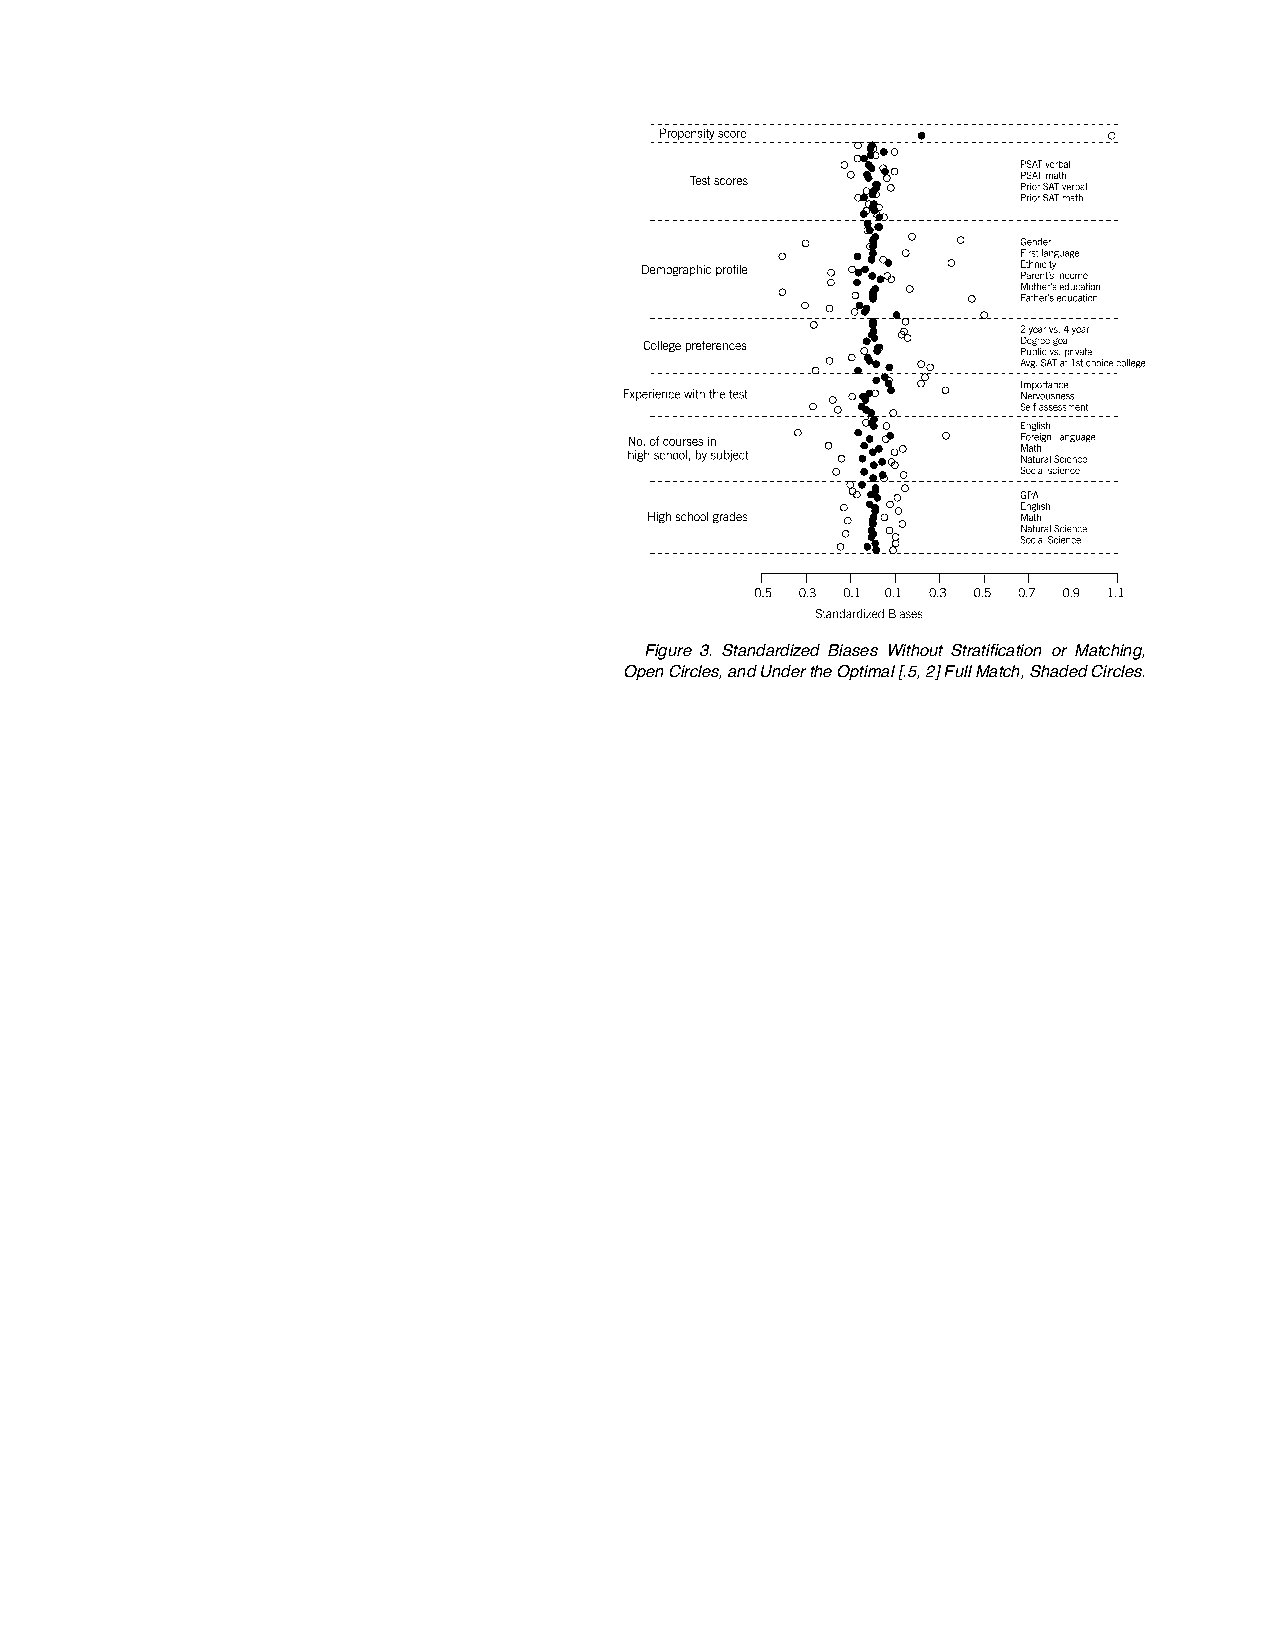
\includegraphics[width = .60 \linewidth]{images/hansen1.pdf}
\end{figure}
\end{frame}

\begin{frame}{Balance Checks}
\begin{figure}[ht] \centering
    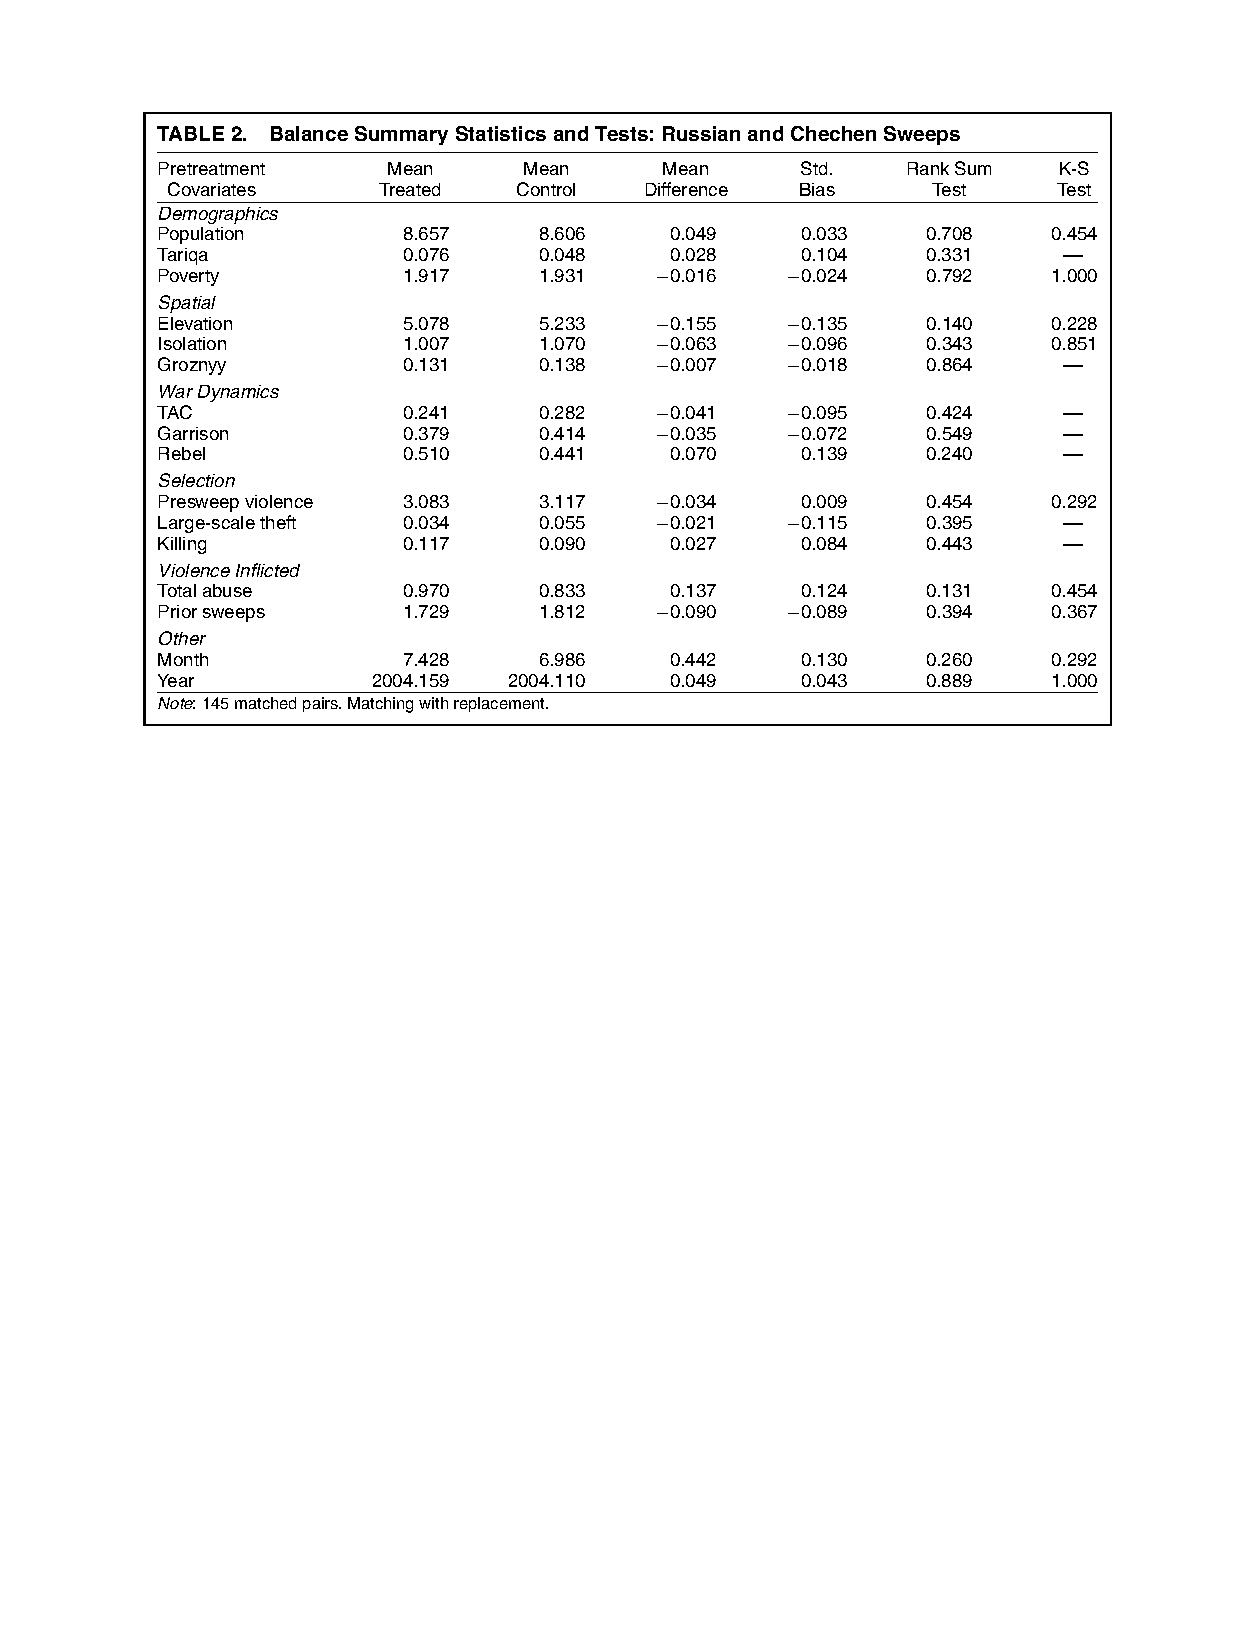
\includegraphics[width = .99 \linewidth]{images/lyall1.pdf}
\end{figure}
\end{frame}

\begin{frame}{Choices when Matching}
\small
\begin{itemize}
\itemsep1pt\parskip0pt\parsep0pt
\item
  With or without replacement? \pause
\item
  How many matches? \pause
\item
  Which matching algorithm?

  \begin{itemize}
  \itemsep1pt\parskip0pt\parsep0pt
  \item genetic matching, kernel matching, full matching
  \item coarsened exact matching
  \item matching as pre-processing
  \item propensity score matching \pause
  \end{itemize}
\item General rule: use whatever gives you the best balance subject to conditioning on what you need and not dropping too many units. \pause %Checking balance is important to get a sense for how much extrapolation is needed
\smallskip
\item Adjustment methods help, but rely on a model to impute missing potential outcomes.
\end{itemize}
\end{frame}



%\begin{frame}{Variance of the Matching Estimator}
%\begin{itemize}
%\itemsep1pt\parskip0pt\parsep0pt
%\item
%  The sampling variance of the matching estimator (conditional on
%  covariates and treatment indicators) can be written as the following:
%  \[ \Var(\hat \tau_{ATT} | \mathbf{X}, \mathbf{D}) = \sum_{i=1}^{N} \lambda_i(\mathbf{X}, \mathbf{W}) \cdot \sigma^2_{D_i}(X_i)\]
%  where $\lambda_i(\mathbf{X}, \mathbf{W})$ is just a set of weights which
%  account for matching with replacement and multiple controls per
%  treatment unit. \pause
%\item
%  $\sigma^2_i$ is the unit level variance. Abadie and Imbens suggest
%  matching to estimate this quantity:
%
%  \begin{itemize}
%  \itemsep1pt\parskip0pt\parsep0pt
%  \item
%    Let $v(i)$ be the closest unit to $i$ with the same treatment
%    indicator ($D_{v(i)} = D_i$). The sample variance of the outcome
%    variable for these 2 units can be used to estimate
%    $\sigma^2_{D_i}(X_i)$:
%    \[ \hat \sigma^2_{D_i}(X_i) = (Y_i - Y_{v(i)})^2 / 2 \] 
%    \item Robust standard errors also available\pause
%  \end{itemize}
%\item Do not use the bootstrap!
%\end{itemize}
%
%\end{frame}
\subsection{Variance Estimation}
\begin{frame}{Variance of the Matching Estimator}
\begin{description}
\item[Option 1.]<1-> Ignore the matching uncertainty and estimate the SEs from whatever model you run on the matched sample
\begin{itemize}
\small
\item treats the matched sample as fixed
\item thus ignores uncertainty in matching
\end{itemize}
\bigskip
\item[Option 2.]<2-> Bootstrap
\begin{itemize}
\small
\item \alert{NO}. Not consistent; ``extreme non-smoothness''
\end{itemize}
\bigskip
\item[Option 3.]<3-> Abadie-Imbens asymptotic SEs
\begin{itemize}
\small
\item uses matched pairs to estimate local variance in $Y_0$ and takes weighted sum that accounts for matching
\item provided by \texttt{Match()} package; widely used.
\end{itemize}
\bigskip
\item[Option 4.]<4-> Post-treatment model SE
\begin{itemize}
\small
\item Use matching to get weights, run weighted regression, cluster robust SEs
\item Default in \texttt{MatchIt} package; good idea to use it.
\end{itemize}
\end{description}
\end{frame}

\subsection{Matching Functions}
\begin{frame}[fragile]{Useful Matching Functions}
\small 
Two packages widely used: \texttt{MatchIt}, and 
\texttt{Matching}.

\onslide<1-> We'll use \texttt{Matching} today (the \texttt{Match} function), but provide \texttt{MatchIt} examples elsewhere.

\footnotesize
\begin{verbatim}
Match(Y = NULL, Tr, X, Z = X, V = rep(1, length(Y)), 
    estimand = "ATT", M = 1, BiasAdjust = FALSE, exact = NULL, 
    caliper = NULL,  replace = TRUE, ties = TRUE, 
    CommonSupport = FALSE, Weight = 1, Weight.matrix = NULL, 
    weights = NULL...) 
\end{verbatim}

Default distance metric is normalized Euclidean distance

\begin{itemize}
\itemsep1pt\parskip0pt\parsep0pt
\item
  \texttt{MatchBalance} for balance checking
\end{itemize}
\end{frame}

\subsection{Example: Blattman and Annan (2009)}
\begin{frame}{Example: Blattman and Annan (2009)}
\small
\begin{quote}
\texttt{The Consequences of
Child Soldiering. \textit{The Review of Economics and Statistics}.}
\end{quote}
\small
\bigskip
\onslide<3-> \textcolor{Blue}{Question}: what is the impact of abduction by the rebel group \textit{Lord's Resistance Army} on education? \\
\bigskip
\onslide<4-> \textcolor{Blue}{ID Strategy:} SOO. According to the logic by which abduction occurred, \emph{we will assume that abduction is indiscriminate, conditional on age and location.}

\footnotesize
\begin{quote}
Abduction was large-scale and seemingly indiscriminate; 60,000 to 80,000 youth are estimated to have been abducted and more than a quarter of males currently aged 14 to 30 in our study region were abducted for at least two weeks...

Youth were typically taken by roving groups of 10 to 20 rebels during night raids on rural homes. Adolescent males appear to have been the most pliable, reliable and effective forced recruits, and so were disproportionately targeted by the LRA. Youth under age 11 and over 24 tended to be avoided and had a high probability of immediate release. 
\end{quote}
\end{frame}

\begin{frame}{Example: Blattman and Annan (2009)}
\small
\onslide<1-> \textcolor{Blue}{Data}: panel survey of male youth in war-afflicted regions of Uganda. \\
\footnotesize
\begin{itemize}
\item \texttt{abd}: abducted by the LRA (the treatment)
\item \texttt{c\_ach -- c\_pal:} Location indicators
\item \texttt{age}: age in years
\item \texttt{fthr\_ed},\texttt{mthr\_ed} : father's/mother's education (years)
\item \texttt{orphan96}: indicator if parent's died before 1997
\item \texttt{hh\_fthr\_frm}: indicator if father is a farmer
\item \texttt{hh\_size96}: household size in 1996
\item \texttt{educ}: years of education
\item \texttt{distress}: index of emotional distress (0-15)
\item \texttt{logwage}: log of average daily wage earned in last 4 weeks
\end{itemize}
\small
\medskip
\onslide<3-> Which of these  \textbf{must} you match on given the ID strategy? \\
\smallskip
\onslide<4-> After matching, which of these should you expect good balance on once  \footnotesize \alert{NB:} \texttt{educ}, \texttt{distress}, and \texttt{logwage} are measured after abduction.\\
\end{frame}

\begin{frame}{Code example(s)}

Check online for example code of matching and balance testing, using both older and newer packages. 

\end{frame}
%\subsection{Propensity Scores}\label{propensity-scores}
%
%%\begin{frame}{Review: Law of Iterated Expectations}
%%
%%\begin{definition}
%%A very important property of conditional expectations is:
%%$$
%%\E[Y]=\E[\E[Y|X]]
%%$$
%%since $\E[Y|X]$ is a function of $X$, the outer expectation
%%is taken with respect to the distribution of $X$.
%%\end{definition}
%%
%%Example: \pause 
%%
%%Imagine $Y$=Support and $X$=gender $(1,0)$. Then, the law of iterated
%%expectations tells us: \[
%%\E[Y]=\pause \E[Y|X=1]\cdot \Pr(X=1) + \E[Y|X=0]\cdot \Pr(X=0).
%%\] This means: \medskip
%%\small
%%
%%\begin{tabular}{lcll}
%%Average Support &=& Average Support for men&$\times$ Proportion of men\\
%%               &+& Average Support for women&$\times$ Proportion of women.
%%\end{tabular}
%%
%%\end{frame}
%
%\begin{frame}{Identification with Propensity Scores}
%
%\begin{definition}
%Propensity score is defined as the selection probability conditional on the confounding variables:
%$\pi(X)=\Pr(D=1|X)$
%\end{definition}
%
%\begin{iass}
%\begin{enumerate}
%\item $(Y_1,Y_0) \indep D |X$ (selection on observables)
%\item $0<\Pr(D=1|X)<1$ with probability one (common support)
%\end{enumerate}
%\end{iass}
%
%\begin{ires}
%Under selection on observables we have $(Y_1,Y_0) \indep D| \pi(X)$, ie. conditioning
%on the propensity score is enough to have independence between the treatment indicator and potential outcomes. Implies substantial dimension reduction.
%\end{ires}
%
%\end{frame}
%
%\begin{frame}{Identification with Propensity Scores}
%
%\begin{Proof}
%\small
%Show that $\Pr(D = 1|Y_0, Y_1, \pi(X)) = \Pr(D = 1|\pi(X)) = \pi(X)$, implying
%independence of $(Y_0,Y_1)$ and $D$ conditional on $\pi(X)$.
%\begin{eqnarray*}
%\Pr(D=1|Y_1,Y_0,\pi(X))&=&\E[D|Y_1,Y_0,\pi(X)]\\ \pause
%&=&\E\left[\E[D|Y_1,Y_0,X]|Y_1,Y_0,\pi(X)\right] \mbox{ (LIE) }\\ \pause
%&=&\E\left[\E[D|X]|Y_1,Y_0,\pi(X)\right] \mbox{ (SOO) } \\\pause
%&=&\E\left[\pi(X)|Y_1,Y_0,\pi(X)\right] \\ \pause
%&=&\pi(X)
%\end{eqnarray*}
%Using a similar argument
%\begin{eqnarray*}
%\Pr(D=1|\pi(X))&=&\E[D|\pi(X)]=\E[\E[D|X]|\pi(x)]\\ \pause
%&=&\E[\pi(X)|\pi(X)]=\pi(X)
%\end{eqnarray*}
%therefore $\Pr(D=1|Y_1,Y_0,\pi(X))=\Pr(D=1|\pi(X))$
%\end{Proof}
%
%\end{frame}
%
%\begin{frame}{Matching on the Propensity Score}
%
%\begin{corollary} If $(Y_1,Y_0) \indep D|X$, then
%\begin{eqnarray*}
%\E[Y|D=1,\pi(X)=\bar{\pi}]-\E[Y|D=0,\pi(X)=\bar{\pi}]&=&\\
%\E[Y_1-Y_0|\pi(X)=\bar{\pi}]
%\end{eqnarray*}
%\end{corollary}
%
%Suggests a two step procedure to estimate causal effects under selection
%on observables:
%
%\begin{enumerate}
%\def\labelenumi{\arabic{enumi}.}
%\itemsep1pt\parskip0pt\parsep0pt
%\item
%  Estimate the propensity score $\pi(X)=P(D=1|X)$ (eg. using
%  logit/probit regression, machine learning methods, etc) \pause
%\item
%  Match or subclassify on propensity score.
%\end{enumerate}
%
%\end{frame}
%
%\begin{frame}{Estimating the Propensity Score}
%
%\begin{itemize}
%\itemsep1pt\parskip0pt\parsep0pt
%\item
%  Given selection on observables we have $(Y_1,Y_0) \indep D|\pi(X)$
%  which implies the balancing property of the propensity score: \[
%    \Pr(X|D=1,\pi(X))=\Pr(X|D=0,\pi(X))
%    \] \pause
%\item
%  We can use this to check if our estimated propensity score actually
%  produces balance:
%  $P(X|D=1,\widehat{\pi}(X))=P(X|D=0,\widehat{\pi}(X))$ \pause
%\item
%  To properly model the assignment mechanism, we need to include
%  important confounders correlated with treatment and outcome
%\item
%  Need to find the correct functional form, miss-specified propensity
%  scores can lead to bias. Any methods can be used (probit, logit, etc.)
%\item
%  Estimate $\mapsto$ Check Balance $\mapsto$ Re-estimate $\mapsto$ Check
%  Balance
%\end{itemize}
%
%\end{frame}
%
%\begin{frame}[fragile]{Example: Blattman (2010)}
%
%\footnotesize
%
%\begin{Shaded}
%\begin{Highlighting}[]
%\NormalTok{pscore.fmla <-}\StringTok{ }\KeywordTok{as.formula}\NormalTok{(}\KeywordTok{paste}\NormalTok{(}\StringTok{"abd~"}\NormalTok{,}\KeywordTok{paste}\NormalTok{(}\KeywordTok{names}\NormalTok{(covar),}\DataTypeTok{collapse=}\StringTok{"+"}\NormalTok{)))}
%\NormalTok{abd <-}\StringTok{ }\NormalTok{data$abd}
%\NormalTok{pscore_model <-}\StringTok{ }\KeywordTok{glm}\NormalTok{(pscore.fmla, }\DataTypeTok{data =} \NormalTok{data, }
%  \DataTypeTok{family =} \KeywordTok{binomial}\NormalTok{(}\DataTypeTok{link =} \NormalTok{logit))}
%\NormalTok{pscore <-}\StringTok{ }\KeywordTok{predict}\NormalTok{(pscore_model, }\DataTypeTok{type =} \StringTok{"response"}\NormalTok{)}
%\end{Highlighting}
%\end{Shaded}
%
%\centering
%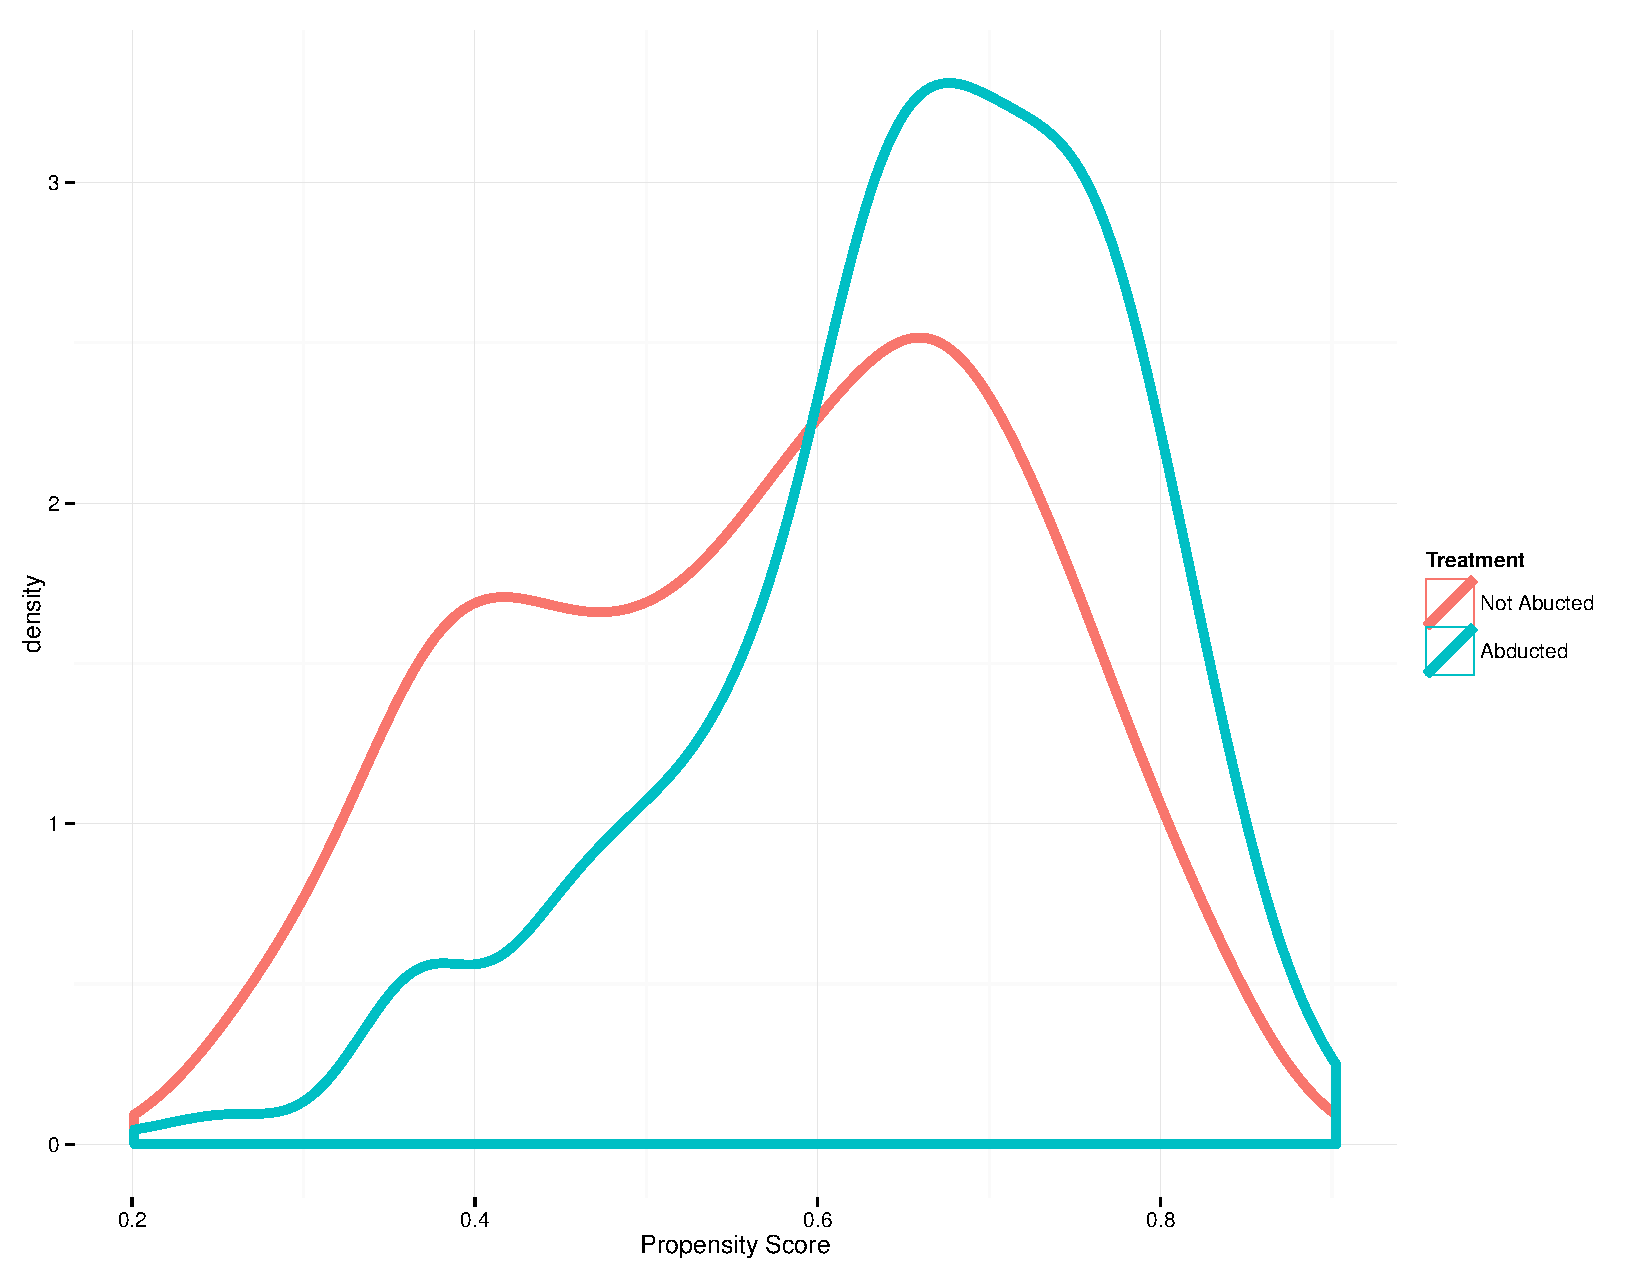
\includegraphics[height = 2.4in]{images/blattman_pscore.pdf}
%
%\end{frame}
%
%\begin{frame}[fragile]{Blattman (2010): Match on the Propensity Score}
%
%\footnotesize
%
%\begin{Shaded}
%\begin{Highlighting}[]
%\NormalTok{match.pscore <-}\StringTok{ }\KeywordTok{Match}\NormalTok{(}\DataTypeTok{Tr=}\NormalTok{abd, }\DataTypeTok{X=}\NormalTok{pscore, }\DataTypeTok{M=}\DecValTok{1}\NormalTok{, }\DataTypeTok{estimand=}\StringTok{"ATT"}\NormalTok{)}
%\end{Highlighting}
%\end{Shaded}
%
%\centering
%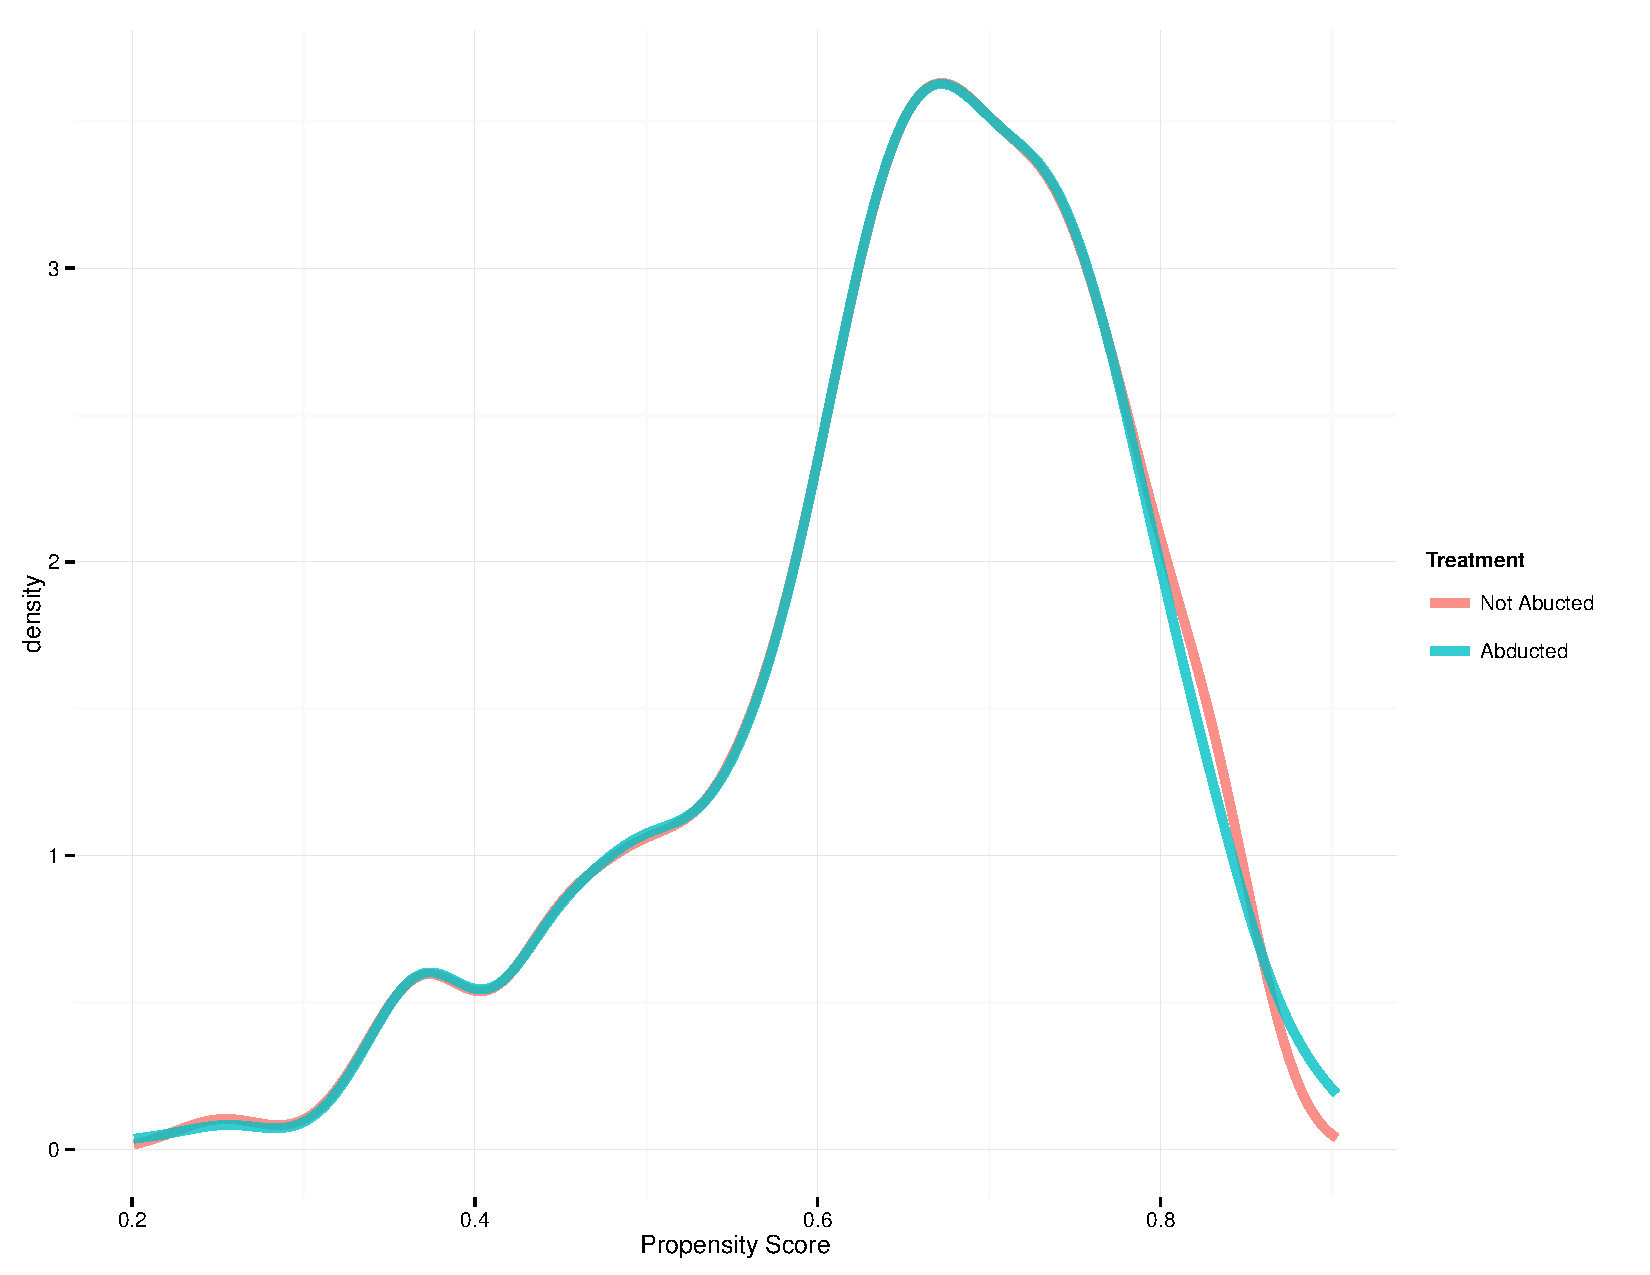
\includegraphics[height = 3in]{images/blattman_pscore_matching.pdf}
%
%\end{frame}
%
%\begin{frame}[fragile]{Blattman (2010): Check Balance}
%
%\footnotesize
%
%\begin{Shaded}
%\begin{Highlighting}[]
%\NormalTok{match.pscore <-}
%\NormalTok{+}\StringTok{ }\KeywordTok{MatchBalance}\NormalTok{(abd ~}\StringTok{ }\NormalTok{age, }\DataTypeTok{data=}\NormalTok{data, }\DataTypeTok{match.out =} \NormalTok{match.pscore)}
%
%\NormalTok{**}\ErrorTok{***}\StringTok{ }\NormalTok{(V1) age **}\ErrorTok{***}
%\StringTok{                       }\NormalTok{Before Matching     After Matching}
%\NormalTok{mean treatment........     }\FloatTok{21.366}          \FloatTok{21.366} 
%\NormalTok{mean control..........     }\FloatTok{20.151}          \FloatTok{20.515} 
%\NormalTok{std mean diff.........     }\FloatTok{24.242}          \FloatTok{16.976} 
%
%\NormalTok{var }\KeywordTok{ratio} \NormalTok{(Tr/Co).....     }\FloatTok{1.0428}         \FloatTok{0.98412} 
%\NormalTok{T-test p-value........  }\FloatTok{0.0012663}       \FloatTok{0.0034409} 
%\NormalTok{KS Bootstrap p-value..      }\FloatTok{0.016}           \FloatTok{0.034} 
%\NormalTok{KS Naive p-value......   }\FloatTok{0.024912}        \FloatTok{0.070191} 
%\NormalTok{KS Statistic..........    }\FloatTok{0.11227}        \FloatTok{0.077899} 
%\end{Highlighting}
%\end{Shaded}
%
%\end{frame}
%
%\begin{frame}[fragile]{Blattman (2010): Mahalanobis Distance Matchng}
%
%\footnotesize
%
%\begin{Shaded}
%\begin{Highlighting}[]
%\NormalTok{match.mah <-}\StringTok{ }\KeywordTok{Match}\NormalTok{(}\DataTypeTok{Tr=}\NormalTok{abd, }\DataTypeTok{X=}\NormalTok{covar, }\DataTypeTok{M=}\DecValTok{1}\NormalTok{, }\DataTypeTok{estimand=}\StringTok{"ATT"}\NormalTok{, }\DataTypeTok{Weight =} \DecValTok{3}\NormalTok{)}
%\KeywordTok{MatchBalance}\NormalTok{(abd ~}\StringTok{ }\NormalTok{age, }\DataTypeTok{data=}\NormalTok{data, }\DataTypeTok{match.out =} \NormalTok{match.mah)}
%
%\NormalTok{**}\ErrorTok{***}\StringTok{ }\NormalTok{(V1) age **}\ErrorTok{***}
%\StringTok{                       }\NormalTok{Before Matching     After Matching}
%\NormalTok{mean treatment........     }\FloatTok{21.366}          \FloatTok{21.366} 
%\NormalTok{mean control..........     }\FloatTok{20.151}          \FloatTok{21.154} 
%\NormalTok{std mean diff.........     }\FloatTok{24.242}          \FloatTok{4.2314} 
%
%\NormalTok{var }\KeywordTok{ratio} \NormalTok{(Tr/Co).....     }\FloatTok{1.0428}          \FloatTok{1.0336} 
%\NormalTok{T-test p-value........  }\FloatTok{0.0012663}      \FloatTok{3.0386e-05} 
%\NormalTok{KS Bootstrap p-value..      }\FloatTok{0.008}           \FloatTok{0.798} 
%\NormalTok{KS Naive p-value......   }\FloatTok{0.024912}         \FloatTok{0.94687} 
%\NormalTok{KS Statistic..........    }\FloatTok{0.11227}        \FloatTok{0.034261} 
%\end{Highlighting}
%\end{Shaded}
%
%\end{frame}
%
%\begin{frame}[fragile]{Blattman (2010): Genetic Matching}
%
%\footnotesize
%
%\begin{Shaded}
%\begin{Highlighting}[]
%\NormalTok{genout <-}\StringTok{ }\KeywordTok{GenMatch}\NormalTok{(}\DataTypeTok{Tr=}\NormalTok{abd,}\DataTypeTok{X=}\NormalTok{covar,}\DataTypeTok{BalanceMatrix=}\NormalTok{covar,}\DataTypeTok{estimand=}\StringTok{"ATT"}\NormalTok{,}
%                  \DataTypeTok{pop.size=}\DecValTok{1000}\NormalTok{)}
%\NormalTok{match.gen <-}\StringTok{ }\KeywordTok{Match}\NormalTok{(}\DataTypeTok{Tr=}\NormalTok{abd, }\DataTypeTok{X=}\NormalTok{covar,}\DataTypeTok{M=}\DecValTok{1}\NormalTok{,}\DataTypeTok{estimand=}\StringTok{"ATT"}\NormalTok{,}\DataTypeTok{Weight.matrix=}\NormalTok{genout)}
%\NormalTok{gen.bal <-}\StringTok{ }\KeywordTok{MatchBalance}\NormalTok{(abd~age,}\DataTypeTok{match.out=}\NormalTok{match.gen,}\DataTypeTok{data=}\NormalTok{covar)}
%
%\NormalTok{**}\ErrorTok{***}\StringTok{ }\NormalTok{(V1) age **}\ErrorTok{***}
%\StringTok{                       }\NormalTok{Before Matching     After Matching}
%\NormalTok{mean treatment........     }\FloatTok{21.366}          \FloatTok{21.366} 
%\NormalTok{mean control..........     }\FloatTok{20.151}          \FloatTok{21.225} 
%\NormalTok{std mean diff.........     }\FloatTok{24.242}          \FloatTok{2.8065} 
%
%\NormalTok{var }\KeywordTok{ratio} \NormalTok{(Tr/Co).....     }\FloatTok{1.0428}          \FloatTok{1.1337} 
%\NormalTok{T-test p-value........  }\FloatTok{0.0012663}         \FloatTok{0.21628} 
%\NormalTok{KS Bootstrap p-value..      }\FloatTok{0.008}           \FloatTok{0.454} 
%\NormalTok{KS Naive p-value......   }\FloatTok{0.024912}         \FloatTok{0.68567} 
%\NormalTok{KS Statistic..........    }\FloatTok{0.11227}        \FloatTok{0.046512} 
%\end{Highlighting}
%\end{Shaded}
%
%\end{frame}
%
%\begin{frame}{Weighting on the Propensity Score}
%
%\small
%Provided that the relevant moments exists, if $Y_1,Y_0\indep D |X$, then
%
%\begin{eqnarray*}
%\tau_{ATE}&=&\E[Y_1-Y_0]=\E\left[
%Y\cdot \frac{D-\pi(X)}{\pi(X)\cdot (1-\pi(X))}
%\right]\\
%\tau_{ATT}&=&\E[Y_1-Y_0|D=1]=\frac{1}{P(D=1)}\cdot \E\left[
%Y\cdot \frac{D-\pi(X)}{1-\pi(X)}
%\right]
%\end{eqnarray*}
%
%\begin{Proof}
%\scriptsize Consider
%\begin{eqnarray*}
%&&\E\left[\left.
%Y \frac{D-\pi(X)}{\pi(X) (1-\pi(X))}\right| X \right]\\
%&=& \E\left[\left.\frac{Y}{\pi(X)} \right|X, D=1 \right] \pi(X) + \E\left[\left.\frac{-Y}{1-\pi(X)}\right|X, D=0\right] (1-\pi(X))\\
%&=& \E[Y|X, D=1] - \E[Y|X, D=0]
%\end{eqnarray*}
%And the results of the proposition follow from integration over $\Pr(X)$ and $\Pr(X|D=1)$.
%\end{Proof}
%
%\end{frame}
%
%\begin{frame}{Weighting on the Propensity Score}
%
%\small
%
%\begin{eqnarray*}
%\tau_{ATE}&=&\E[Y_1-Y_0]=\E\left[
%Y\cdot \frac{D-\pi(X)}{\pi(X)\cdot (1-\pi(X))}
%\right]\\
%\tau_{ATT}&=&\E[Y_1-Y_0|D=1]=\frac{1}{\Pr(D=1)}\cdot \E\left[
%Y\cdot \frac{D-\pi(X)}{1-\pi(X)}
%\right]
%\end{eqnarray*}
%
%How do we estimate this? \pause Analogy principle suggest a two step
%procedure:
%
%\begin{enumerate}
%\def\labelenumi{\arabic{enumi}.}
%\itemsep1pt\parskip0pt\parsep0pt
%\item
%  Estimate the propensity score ($\widehat{\pi}(X)$)
%\item
%  Use sample averages and the estimated propensity score to produce
%  analog estimators of $\tau_{ATE}$ and $\tau_{ATT}$:
%
%  \begin{eqnarray*}
%  \widehat{\tau}_{ATE}&=&\frac{1}{N} \sum_{i=1}^N
%  Y_i\cdot \frac{D_i-\widehat{\pi}(X_i)}{\widehat{\pi}(X_i)\cdot
%  (1-\widehat{\pi}(X_i))},\\
%  \widehat{\tau}_{ATT}&=&\frac{1}{N} \sum_{i=1}^N
%  Y_i\cdot \frac{D_i-\widehat{\pi}(X_i)}{1-\widehat{\pi}(X)}
%  \end{eqnarray*}
%\end{enumerate}
%
%\end{frame}
%
%\begin{frame}[fragile]{Blattman (2010): Weighting on the Propensity
%Score}
%
%\begin{Shaded}
%\begin{Highlighting}[]
%\KeywordTok{mean}\NormalTok{(covar$age[abd ==}\StringTok{ }\DecValTok{1}\NormalTok{]) -}\StringTok{ }\KeywordTok{mean}\NormalTok{(covar$age[abd ==}\StringTok{ }\DecValTok{0}\NormalTok{])}
%\NormalTok{[}\DecValTok{1}\NormalTok{] }\FloatTok{1.215263}
%
%\KeywordTok{sum}\NormalTok{(covar$age *}\StringTok{ }\NormalTok{(abd -}\StringTok{ }\NormalTok{pscore) /}\StringTok{ }\NormalTok{(}\DecValTok{1} \NormalTok{-}\StringTok{ }\NormalTok{pscore)) /}\StringTok{ }\KeywordTok{length}\NormalTok{(abd)}
%\NormalTok{[}\DecValTok{1}\NormalTok{] }\FloatTok{0.007663878}
%\end{Highlighting}
%\end{Shaded}
%
%\end{frame}
%
%%\begin{frame}{Caveats about Inverse Propensity Score Weighting}
%%
%%\begin{itemize}
%%\itemsep1pt\parskip0pt\parsep0pt
%%\item
%%  Shown to have poor finite sample performance when some weights are
%%  ``extreme'', which indicates a lack of overlap (Kang and Schaefer
%%  2008).
%%\item
%%  Might want to trim units from the sample with extreme weights, though
%%  this will change your estimand. See Crump, Hotz, Imbens, and Mitnik
%%  (2009) for more on this. \pause
%%\item
%%  \textbf{Entropy Balancing}: To avoid the iterative process of PS
%%  weighting and matching, choose weights that optimize for balance
%%  directly (Hainmueller 2011).
%%\end{itemize}
%%
%%\end{frame}



\end{document}